\documentclass{article}

% if you need to pass options to natbib, use, e.g.:
    \PassOptionsToPackage{numbers, compress}{natbib}
% before loading neurips_2018

% ready for submission
% \usepackage{neurips_2018}

% to compile a preprint version, e.g., for submission to arXiv, add add the
% [preprint] option:
\usepackage[preprint]{nips_2018}

% to compile a camera-ready version, add the [final] option, e.g.:
     %\usepackage[final]{neurips_2018}

% to avoid loading the natbib package, add option nonatbib:
%     \usepackage[nonatbib]{neurips_2018}

\usepackage[utf8]{inputenc} % allow utf-8 input
\usepackage[T1]{fontenc}    % use 8-bit T1 fonts
\usepackage{hyperref}       % hyperlinks
\usepackage{url}            % simple URL typesetting
\usepackage{booktabs}       % professional-quality tables
\usepackage{amsfonts}       % blackboard math symbols
\usepackage{nicefrac}       % compact symbols for 1/2, etc.
\usepackage{microtype}      % microtypography
\usepackage{natbib}
\usepackage{color}
\usepackage{amsmath}
\usepackage{amsthm}
\usepackage{graphicx}
\usepackage[ruled]{algorithm2e}
\usepackage{bbm}
\usepackage{subcaption}
\usepackage{caption}
\usepackage{array}
\newcolumntype{P}[1]{>{\centering\arraybackslash}p{#1}}

\SetKwInput{kwInit}{Init}
\newtheorem*{remark}{Remark}

\DeclareMathOperator*{\argmin}{arg\,min}
\DeclareMathOperator*{\argmax}{arg\,max}
\newtheorem{theorem}{Theorem}
%\newtheorem{theorem}{Theorem}[section]
\newtheorem{proposition}[theorem]{Proposition}
\newtheorem{lemma}{Lemma}
\newtheorem{corollary}[theorem]{Corollary}
\newtheorem{definition}[theorem]{Definition}
\newtheorem{assumption}[theorem]{Assumption}

\newcommand{\RSA}{\mathbb{R}^{|\mathcal{S}|\times|\mathcal{A}|}}
\newcommand{\RSAvector}{\mathbb{R}^{|\mathcal{S}||\mathcal{A}| \times 1}}
\newcommand{\RS}{\mathbb{R}^{|\mathcal{S}|}}
\newcommand{\Rvector}[1]{\mathbb{R}^{#1}}
\newcommand{\Rmatrix}[2]{\mathbb{R}^{#1 \times #2}}
\newcommand{\AdaBracket}[1]{\left(#1\right)}
\newcommand{\AdaRectBracket}[1]{\left[#1\right]}
\newcommand{\AdaAngleBracket}[1]{\left\langle#1\right\rangle}
\newcommand{\AdaAngleProduct}[2]{\left\langle#1, #2\right\rangle}
\newcommand{\chiAny}[3]{\chi^{#1}\AdaBracket{#2||#3}}
\newcommand{\expectation}[2]{\mathbb{E}_{#1}\AdaRectBracket{#2}}
\newcommand{\qlog}{$q$-logarithm }
\newcommand{\qexp}{$q$-exponential }
\newcommand{\fdiv}{$f$-divergence }
\newcommand{\qstarlog}{$q^*$-logarithm }
\newcommand{\qstarexp}{$q^*$-exponential }
\newcommand{\tsallis}[1]{S_q(#1)}
\newcommand{\sparse}[1]{S_2(#1)}
\newcommand{\qKL}{D^{q}_{\!K\!L}\!\AdaBracket{\pi || \bar{\pi}}}
\newcommand{\qKLindex}[2]{D^{q}_{\!K\!L}\!\AdaBracket{\pi_{#1}|| \pi_{#2}}}
\newcommand{\qstarKLindex}[2]{D^{q^*}_{\!K\!L}\!\AdaBracket{\pi_{#1}|| \pi_{#2}}}
\newcommand{\qKLany}[2]{D^{q}_{\!K\!L}\!\left(#1 \left|  \right| #2 \right)}
\newcommand{\qKLstarany}[2]{D^{q^*}_{\!K\!L}\!\left(#1 \left|  \right| #2 \right)}
\newcommand{\KL}{D_{\!K\!L}\!\AdaBracket{\pi || \bar{\pi}}}
\newcommand{\KLindex}[2]{D_{\!K\!L}\!\AdaBracket{\pi_{#1}|| \pi_{#2}}}
\newcommand{\KLany}[2]{D_{\!K\!L}\!\left(#1 \left|  \right| #2 \right)}
\newcommand{\entropy}{\mathcal{H}\left( \pi \right)}
\newcommand{\entropyany}[1]{\mathcal{H}\left( #1 \right)}
\newcommand{\entropyIndex}[1]{\mathcal{H}\left( \pi_{#1} \right)}
\newcommand{\fdivany}[2]{D_{f}\!\left(#1 \left|  \right| #2 \right)}
\newcommand{\logq}[1]{\ln_{q}\!#1}
\newcommand{\logstarq}[1]{\ln_{q^*}\!#1}
\newcommand{\expq}[1]{\exp_{q}\!#1}
\newcommand{\expstarq}[1]{\exp_{q^*}\!#1}
\newcommand{\eq}[1]{Eq.\,(#1)}
\newcommand{\taulogqratio}[3]{\mathbb{M}_{#1,#2} + \ln_{#3}{\pi}_{#1}}
\newcommand{\uniformA}{\left|\mathcal{A}\right|}
\newcommand{\normalization}[1]{\tau\psi\AdaBracket{ \frac{Q_{#1}}{\tau}}}
\newcommand{\renyi}{Rényi }
\newcommand{\renyidivany}[2]{D_\text{\renyi}\!\!\AdaBracket{ #1 || #2}}
\newcommand{\transition}{\gamma P_{\pi}}
\newcommand{\greedy}[1]{\argmax_{\pi}\!\AdaAngleProduct{\pi}{#1}}
\newcommand{\greedyH}[1]{\argmax_{\pi}\!\AdaAngleProduct{\pi}{#1 - \tau\ln\pi}}
\newcommand{\greedyOmega}[1]{\argmax_{\pi}\!\AdaBracket{\AdaAngleProduct{\pi}{#1} - \tau\Omega(\pi)}}
\newcommand{\greedyTKL}[1]{\argmax_{\pi}\!\AdaAngleProduct{\pi}{#1 - \ln_{{q}}\!\frac{\pi}{\pi_k}}}
\newcommand{\BellmanKL}[2]{T^{\lambda,0}_{\pi_{#1}|\pi_{#2}}}
\newcommand{\BellmanKLGreek}[3]{T^{#1,0}_{\pi_{#2}|\pi_{#3}}}
\newcommand{\BellmanKLbar}{T^{\lambda, 0}_{\pi|\bar{\pi}}}
\newcommand{\BellmanH}[2]{r + \gamma P\!\AdaAngleProduct{\pi_{#1}}{Q_{#2} -
\tau\ln\pi_{#1}}}
\newcommand{\BellmanOmega}[2]{r + \gamma P\!\AdaBracket{ \AdaAngleProduct{\pi_{#1}}{Q_{#2}} - \tau\Omega(\pi_{#1})}}
\newcommand{\BellmanTKL}[2]{r + \gamma P\!\AdaAngleProduct{\pi_{#1}}{\TsallisQ{#2} - \ln_{q}\!\frac{\pi_{#1}}{\pi_{#2}}}}
\newcommand{\BellmanImplicit}[2]{\tilde{T}^{0,#1}_{\pi_{#2}}}
\newcommand{\BellmanBoth}[4]{{T}^{#1,#2}_{\pi_{#3}|\pi_{#4}}}
\newcommand{\BellmanG}[1]{T^{\alpha}_{\pi_{#1}}}
\newcommand{\Bellman}[1]{r + \gamma P_* Q_{#1} }
\newcommand{\sumJK}[1]{\sum_{j=#1}^{k}}
\newcommand{\datasetQ}{Q_{\pi_{\mathcal{D}}}}
\newcommand{\datasetOptimalQ}{Q_{*, \pi_{\mathcal{D}}}}
\newcommand{\datasetPolicy}{\pi_{\mathcal{D}}}


\title{Offline Reinforcement Learning with Tsallis Regularization}

% The \author macro works with any number of authors. There are two commands
% used to separate the names and addresses of multiple authors: \And and \AND.
%
% Using \And between authors leaves it to LaTeX to determine where to break the
% lines. Using \AND forces a line break at that point. So, if LaTeX puts 3 of 4
% authors names on the first line, and the last on the second line, try using
% \AND instead of \And before the third author name.

\author{%
  Department of Computing Science\\
  Alberta University\\
  Pittsburgh, PA 15213 \\
  \texttt{hippo@cs.cranberry-lemon.edu} \\
  % examples of more authors
  % \And
  % Coauthor \\
  % Affiliation \\
  % Address \\
  % \texttt{email} \\
  % \AND
  % Coauthor \\
  % Affiliation \\
  % Address \\
  % \texttt{email} \\
  % \And
  % Coauthor \\
  % Affiliation \\
  % Address \\
  % \texttt{email} \\
  % \And
  % Coauthor \\
  % Affiliation \\
  % Address \\
  % \texttt{email} \\
}

\begin{document}
% \nipsfinalcopy is no longer used

\maketitle

\begin{abstract}
    We show that the Tsallis regularization is well suited to offline reinforcement learning, where its main drawback insufficient exploration vanishes.
    Furthermore, Tsallis entropy induces sparsemax policies which have a natural interpretation of regarding actions not present in the dataset as the truncated actions, hence no support constraint as is done in In-Sample softmax is necessary.
\end{abstract}


\section{Introduction}





\section{Background}


We focus on discrete-time discounted Markov Decision Processes (MDPs) expressed by the tuple $(\mathcal{S}, \mathcal{A}, P,  r,  \gamma)$, where $\mathcal{S}$ and $\mathcal{A}$ denote state space and finite action space, respectively. 
$d(\cdot)$ denotes the initial state distribution.
$P(\cdot |s,a)$ denotes transition probability over the state space given state-action pair $(s,a)$,  
and $r(s,a)$ defines the reward associated with that transition. 
When time step $t$ is of concern, we write $r_t := r(s_t, a_t)$.
$\gamma \in (0,1)$ is the discount factor.
A policy $\pi(\cdot|s)$ is a mapping from the state space to distributions over actions.
% The stationary state distribution induced by $\pi$ can then be defined as $d^{\pi}_{\mu}(s)\!:=\!(1-\gamma)\sum^{\infty}_{t=0}\gamma^{t}P(s_t=s|\pi, \mu)$.
We define the state value function at a specific state $s$ following policy $\pi$  as  $V_{\pi}(s) = \mathbb{E}\AdaRectBracket{\sum_{t=0}^{\infty} r_t | s }$.
Likewise, we define the state-action value function given initial action $a_0$ as  $Q_{\pi}(s,a) = \mathbb{E}\AdaRectBracket{\sum_{t=0}^{\infty} r_t | s_0=s, a_0 = a }$,
% \begin{align}
%     Q_{\pi}(s,a) = \mathbb{E}\AdaRectBracket{\sum_{t=0}^{\infty} r_t | s_0=s, a_0 = a } ,
% \end{align}
where the expectation is with respect to the policy $\pi$ and transition probability $P$.


A standard approach to find the optimal value function $Q_*$ is value iteration. To define the formulas for value iteration, it will be convenient to write these functions as vectors, $V_{\pi} \in \RS$ and $Q_{\pi} \!\in\! \RSA$. 
For notational convenience, we define the inner product for any two functions $F_1,F_2\in\RSA$  as $\AdaAngleProduct{F_1}{F_2} \in \RS$, where we only take the inner product over actions. 
% MARTHA: mention this when it is used
%$\boldsymbol{1}$ denotes an all-one vector whose dimension should be clear from the context.
The Bellman operator acting upon any function $Q \!\in\! \RSA$ can be defined as: $T_{\pi}Q := r + \transition Q$, where $P_{\pi}Q \!\in\! \RSA \!:=\! \mathbb{E}_{s'\sim P(\cdot|s,a),a'\sim\pi(\cdot|s')}\!\AdaRectBracket{Q(s',a')} \!=\! P\!\AdaAngleProduct{\pi}{Q}$.
When $\pi$ is greedy with respect to $Q$, we have the Bellman optimality operator defined by $T_*Q := r + \gamma P_* Q$, $P_*Q \!=\! \mathbb{E}_{s'\sim P(\cdot|s,a)}\!\AdaRectBracket{\max_{a'}Q(s',a')}$. 
The above definitions should be understood as component-wise.
Repeatedly applying the Bellman operator $T_{\pi}Q$ converges to the unique fixed point $Q_{\pi}$, and $T_*Q$ it converges to the optimal action value function $Q_*:=Q_{\pi^*}$.
% Typically the Bellman operator is applied $m \geq 1$ times, and
% $m=1,\infty$ corresponds value iteration and policy iteration, respectively.
% $1\!<\! m < \!\infty\!$ implies the use of approximate modified policy iteration \citep{scherrer15-AMPI}.
This basic recursion can be modified with the addition of a regularizer $\Omega(\pi)$:
\begin{align}
    \begin{cases}
        \pi_{k+1} = \greedy{Q_{k}}, & \\
        Q_{k+1} =  \AdaBracket{ T_{\pi_{k+1}} Q_k }^m , &
    \end{cases}
    \label{eq:PI}
\quad
    \begin{cases}
        \pi_{k+1} = \greedyOmega{Q_{k}}, & \\
        Q_{k+1} = \AdaBracket{T_{\pi_{k+1, \Omega}}Q_k}^m &
    \end{cases}
\end{align}
% MARTHA: What? why would m = infty be policy iteration? this formulas has T_*
%
% \begin{align}
%   \begin{cases}
%       \pi_{k+1} = \greedyOmega{Q_{k}}, & \\
%       Q_{k+1} = \AdaBracket{T_{\pi_{k+1, \Omega}}Q_k}^m &
%   \end{cases}
%   \label{eq:regularizedPI}
% \end{align}
where $T_{\pi_{k+1}, \Omega}Q_k \!=\! \BellmanOmega{k+1}{k}$ is the regularized Bellman operator \citep{geist19-regularized}. This modified recursion is guaranteed to converge if $\Omega$ is concave in $\pi$. For standard (Shannon) entropy regularization, we use $\Omega(\pi) = -\entropy = \AdaAngleProduct{\pi}{\ln\pi}$. The resulting optimal policy has $\pi_{k+1} \propto \exp\AdaBracket{\tau^{-1}Q_k}$, where $\propto$ indicates \emph{proportional to} up to a constant not depending on actions.

Another popular choice is KL divergence $\Omega(\pi)=\KLany{\pi}{\mu} = \AdaAngleProduct{\pi}{\ln{\pi} \!-\!\ln{\mu}}$, which is more general since we recover Shannon entropy when we choose $\mu$ to be a uniform distribution, i.e. $\frac{1}{|\mathcal{A}|}$. In this work, when we say KL regularization, we mean the standard choice of setting $\mu = \pi_k$, the estimate from the previous update.
Therefore, $D_\text{KL}$ serves as a penalty to penalize aggressive policy changes.
The optimal policy in this case takes the form $\pi_{k+1}\propto\pi_k\exp\AdaBracket{\tau^{-1} Q_k}$.
By induction, we can show this KL-regularized optimal policy $\pi_{k+1}$ is a softmax over a uniform average over the history of action value estimates \cite{vieillard2020leverage}:
\begin{align}
  \pi_{k+1} \propto \pi_k \exp\AdaBracket{\tau^{-1} Q_k}  \propto \cdots \propto \exp\AdaBracket{\! \tau^{-1}\sumJK{1}Q_j}
  .
  \label{eq:average}
\end{align}
Using KL regularization has been shown to be theoretically superior to entropy regularization, in terms of error tolerance \cite{azar2012dynamic,vieillard2020leverage,Kozuno-2022-KLGenerativeMinMaxOptimal,chan2021-greedification}.

The definitions of $\mathcal{H}(\cdot)$ and $D_\text{KL}(\cdot||\cdot)$ rely on the standard logarithm and its inverse (the exponential) and both induce softmax policies as an exponential over (weighted) action-values \citep{hiriart2004-convexanalysis,Nachum2020-RLFenchelRockafellar}. 
Convergence properties of the resulting regularized algorithms have been well studied \citep{kozunoCVI,geist19-regularized,vieillard2020leverage}.
In this paper, we investigate Tsallis entropy and Tsallis KL divergence as the regularizer, which generalize Shannon entropy and KL divergence respectively.



\section{$q$-statistics and Tsallis regularization}


\begin{figure}
    \centering
    \begin{subfigure}[b]{0.3\textwidth}
        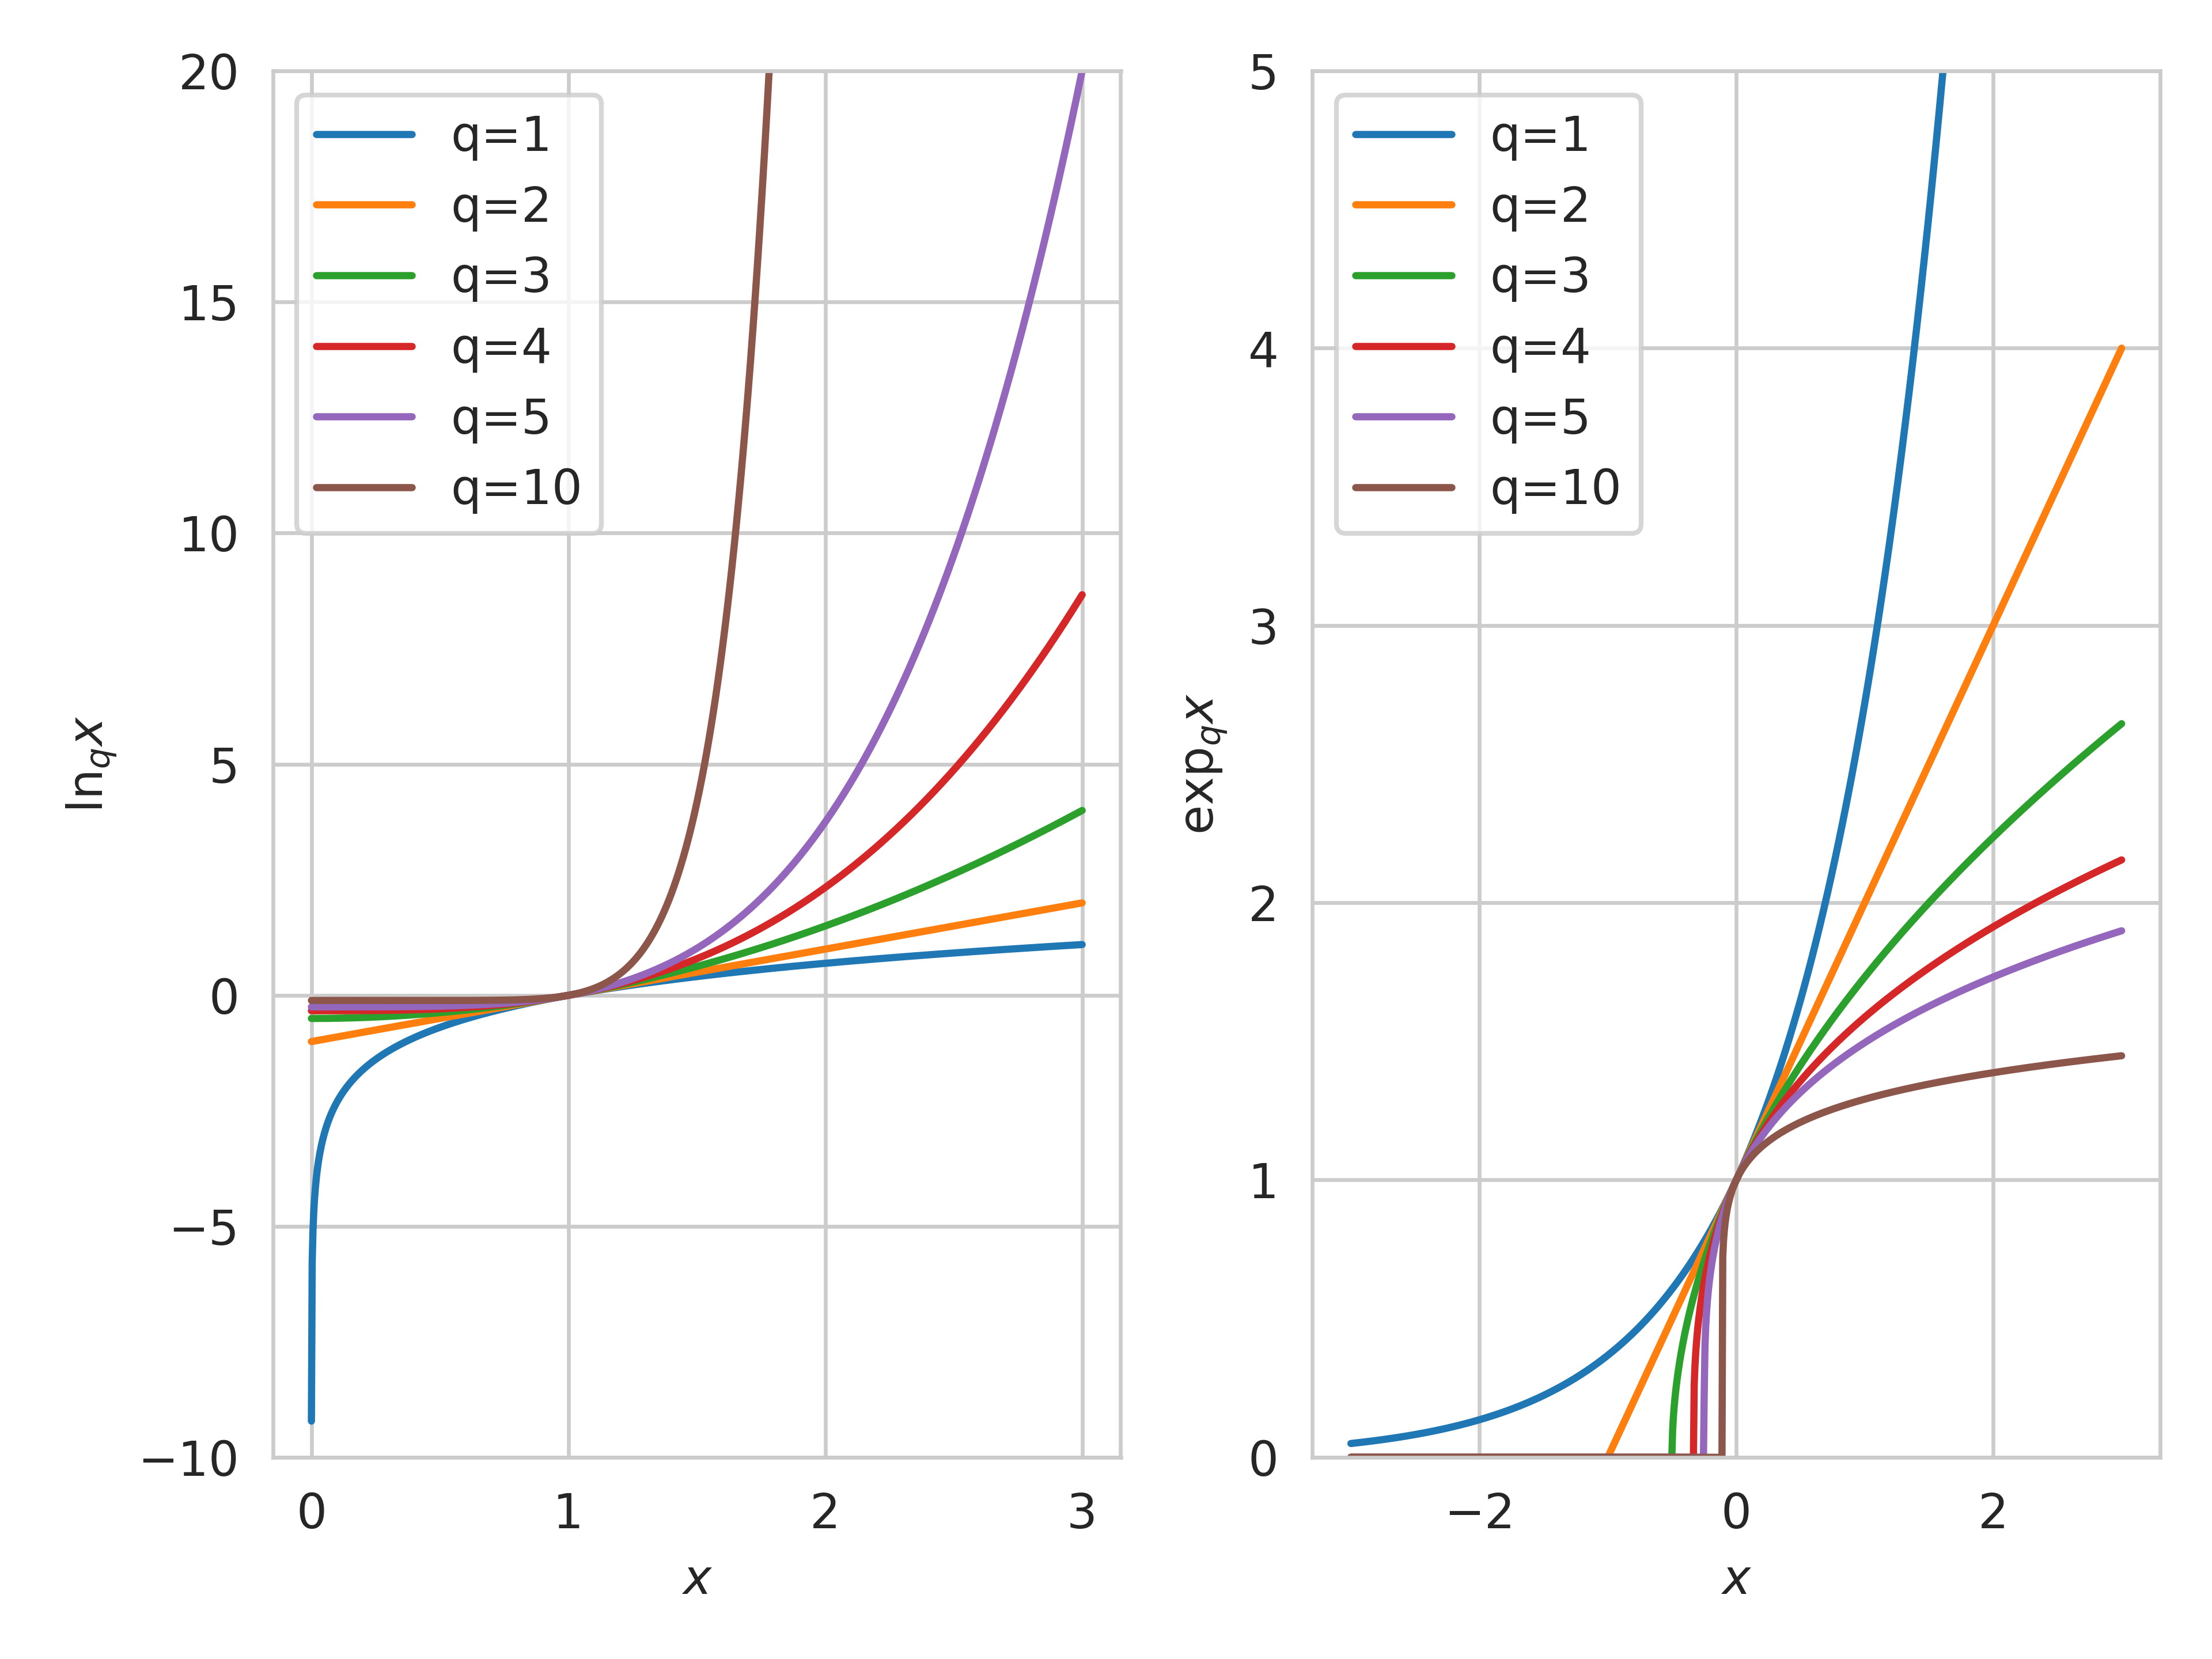
\includegraphics[width=\textwidth]{img/q_stat_illus.png}
    \end{subfigure}
    \begin{subfigure}[b]{0.3\textwidth}
        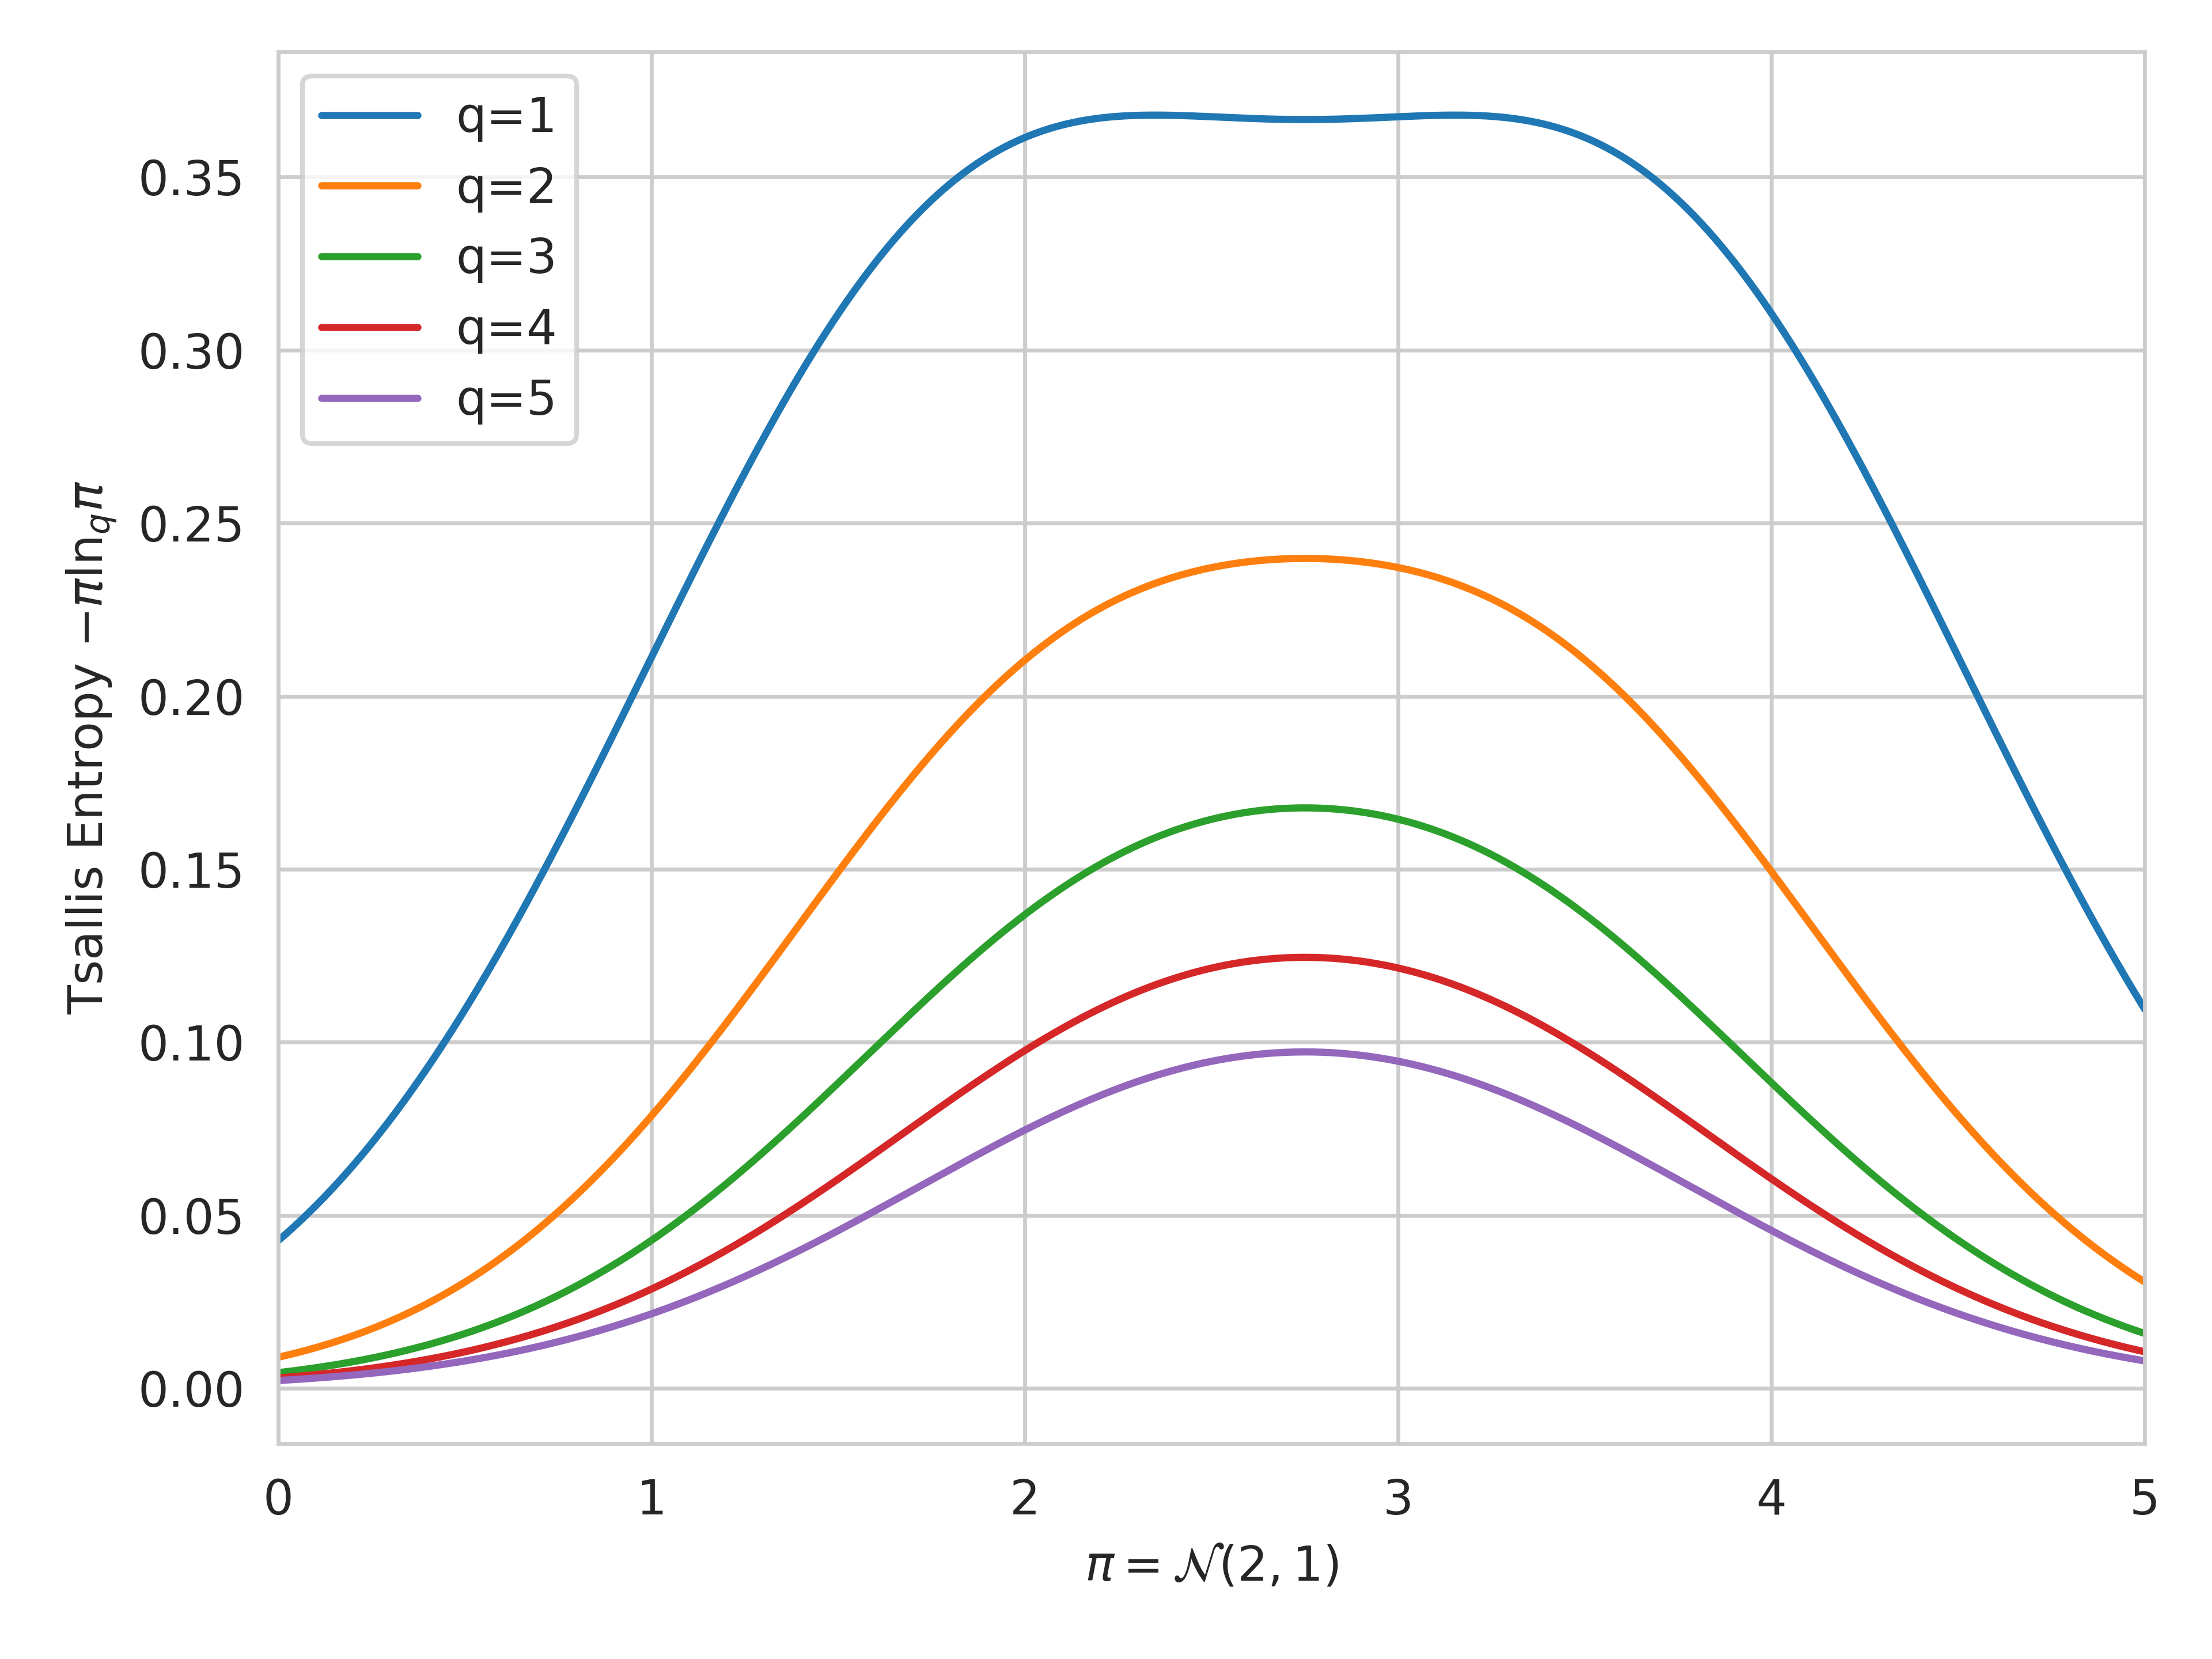
\includegraphics[width=\textwidth]{img/tsallis_entropy.png}
    \end{subfigure}
    \begin{subfigure}[b]{0.3\textwidth}
        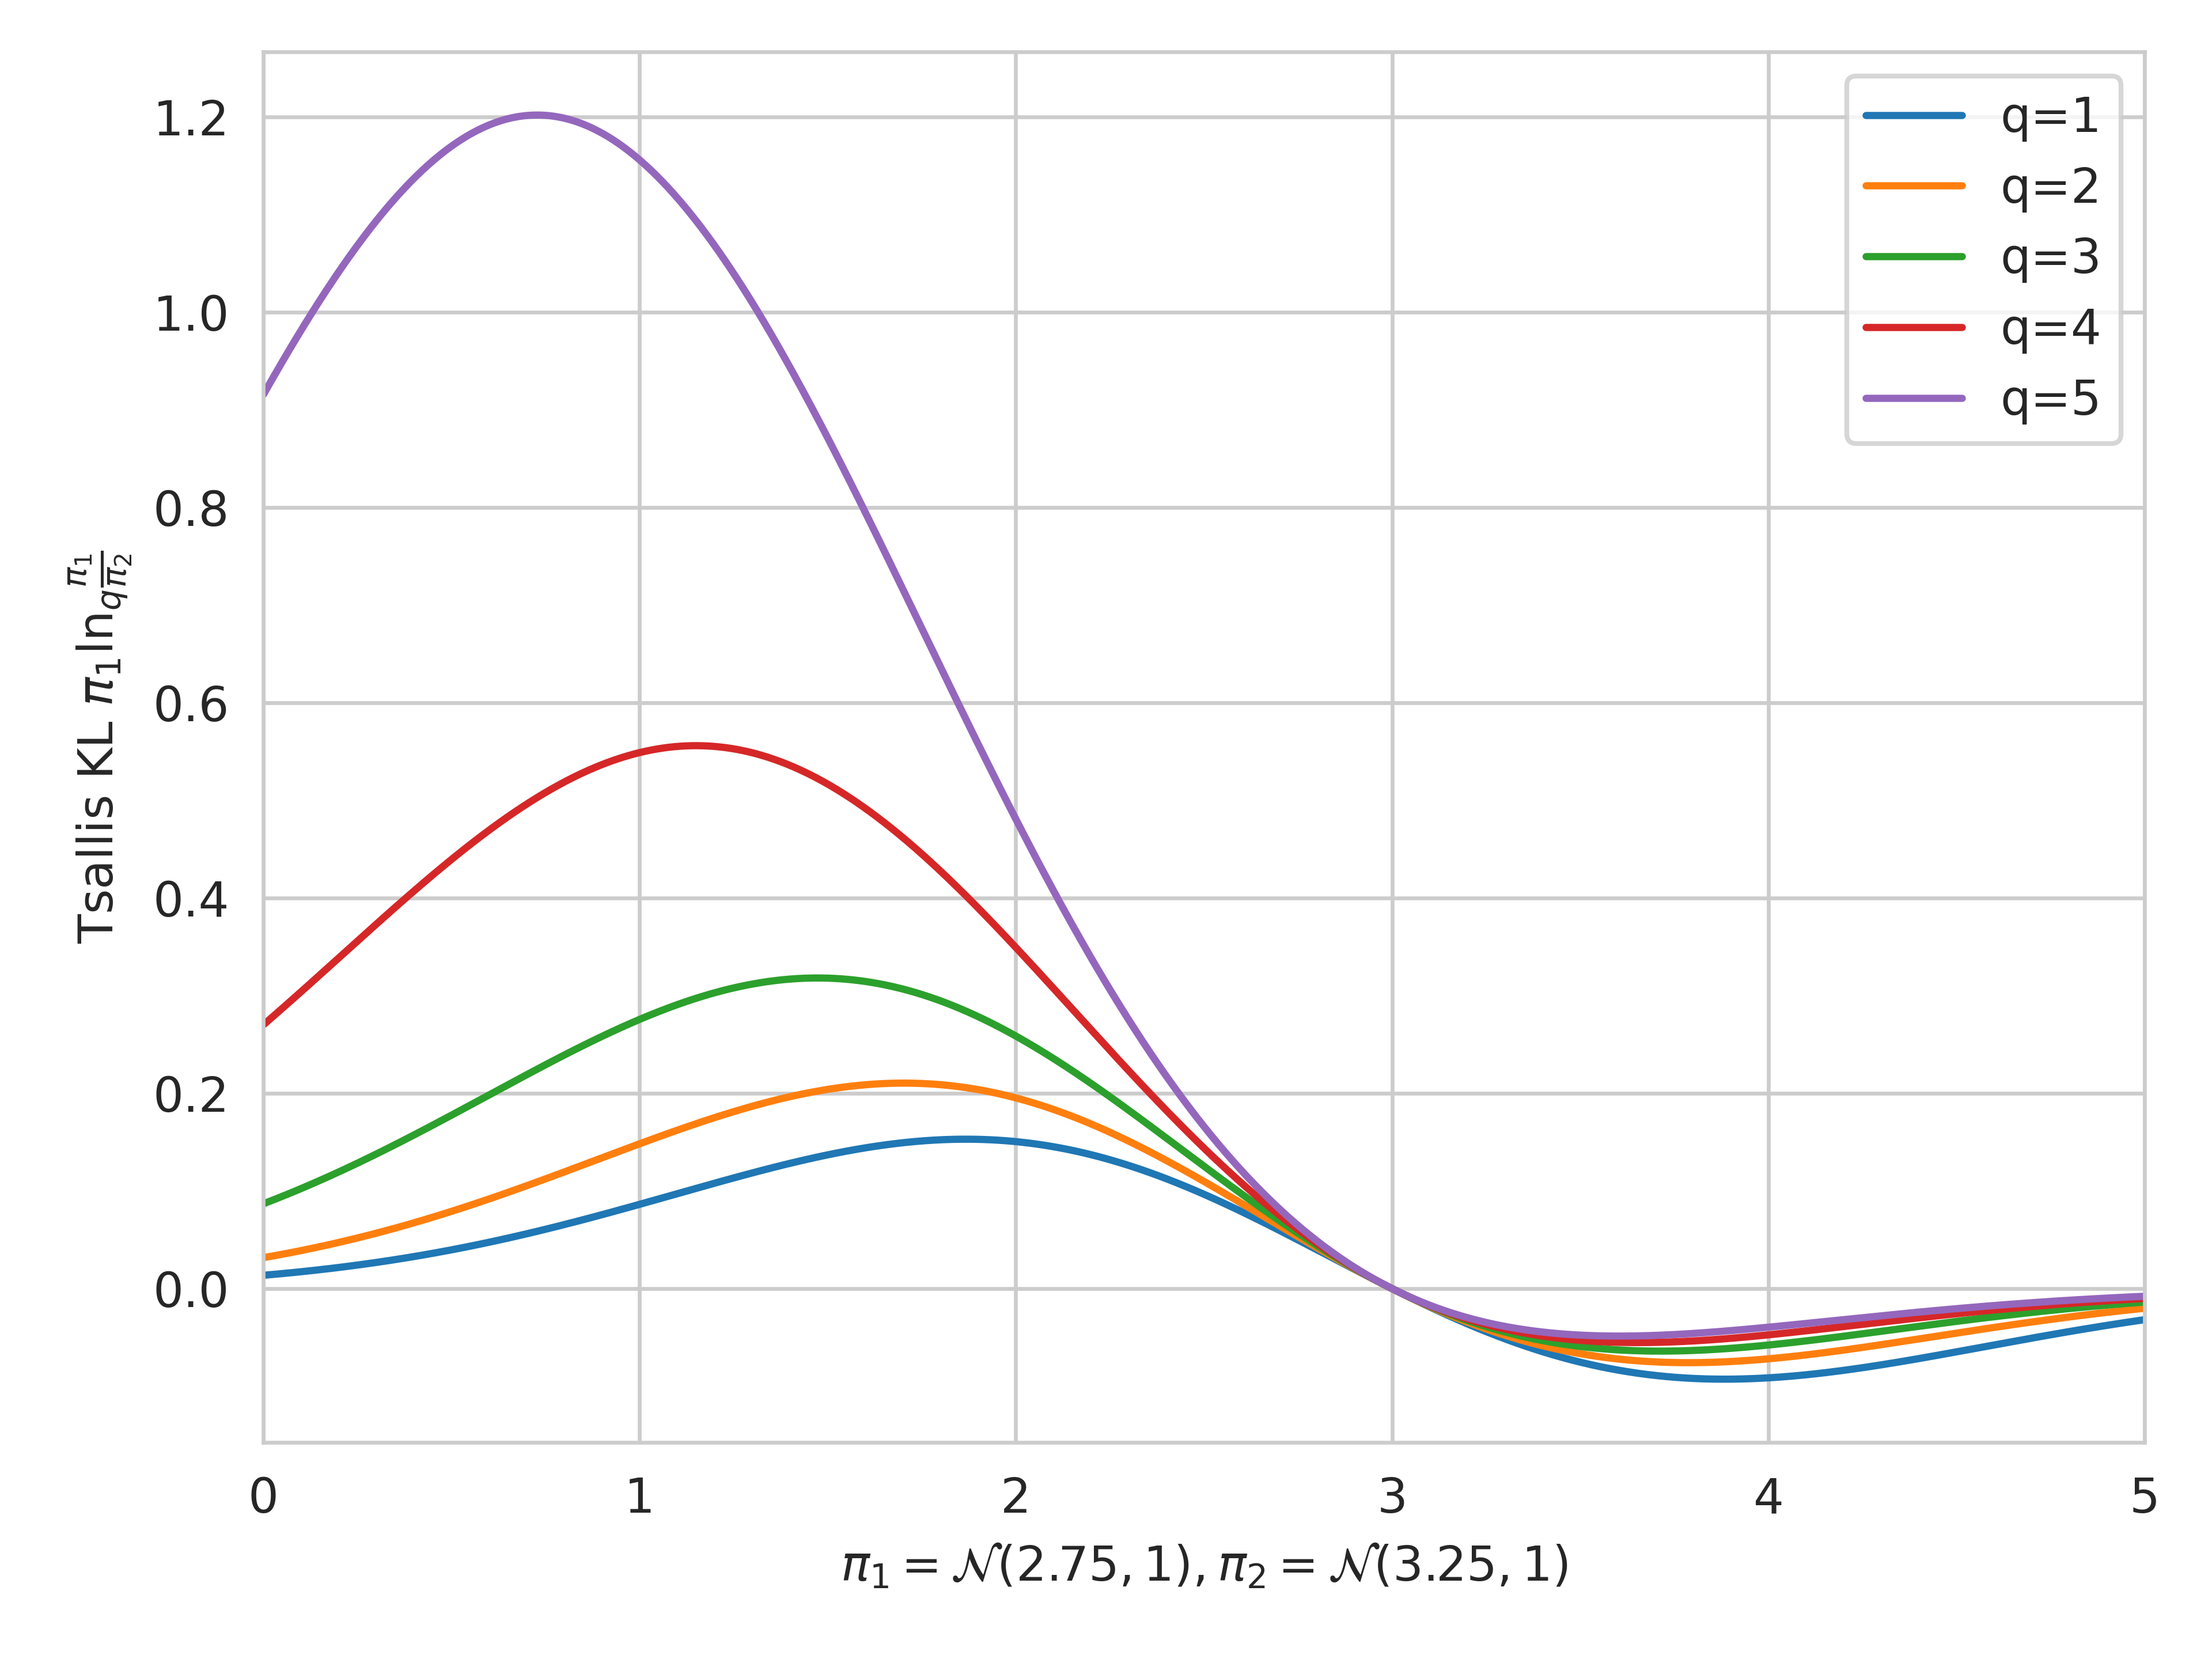
\includegraphics[width=\textwidth]{img/tsallis_kl.png}
    \end{subfigure}
    \caption{(Left) Behavior of \qlog and $q$-exponential functions.
    When $q=1$ they respectively recover the standard logarithm and exponential.
    (Mid) Tsallis entropy of the Gaussian policy $\mathcal{N}(2, 1)$. (Right) Tsallis KL divergence between two Gaussian policies $\mathcal{N}(2.75, 1)$ and $\mathcal{N}(3.25, 1)$.
    }
    \label{fig:q_stats}
\end{figure}

A more general form of entropy known as Tsallis entropy is proposed by \cite{TsallisEntropy},  defined based on the \qlog that is referred to as \emph{deformed logarithm} \cite{tsallis2009introduction}.
Let us revisit the definition of \qlog its unique inverse function $q$-exponential (analogous to the exponential function), see Figure \ref{fig:q_stats}.
We can define the Tsallis entropy $S_q(\pi)$ in a similar way to Shannon entropy with \qlog:
\begin{align}
    \begin{split}
        q \in  \mathbb{R}, \quad \logq{x} = \frac{x^{q-1} - 1}{q-1}, \quad \expq{x} = \AdaRectBracket{1 + (q - 1)x}^{\frac{1}{q-1}}_{+},\quad \tsallis{\pi} = -\AdaAngleProduct{\pi}{\logq{\pi}}.
    \end{split}
\end{align}
When $q=2$, we recover the Tsallis sparse entropy \cite{Martins16-sparsemax}, which achieves the sparsity by projecting onto the probability simplex \cite{Blondel-2020LearningFenchelYoundLoss}.
In RL, it has been investigated by \cite{Lee2018-TsallisRAL,Lee2020-generalTsallisRSS} and it is known that the optimal regularized policy takes the form:
\begin{align*}
    &\pi_{k+1}(a|s) = \AdaRectBracket{\frac{Q_k(s,a)}{\tau} - \psi\AdaBracket{\frac{Q_k(s, \cdot)}{\tau}}}_{+} = \exp_2 \AdaBracket{\frac{Q_k(s,a)}{\tau } - \tilde{\psi}\AdaBracket{\frac{Q_k(s, \cdot)}{\tau }}}, \\
    &{\psi}\AdaBracket{\frac{Q_{k}(s,\cdot)}{\tau}} \doteq \frac{\sum_{a\in K(s)} \frac{Q(s,a)}{\tau} - 1 }{|K{(s)}|}, \,\, \tilde{\psi}\AdaBracket{\frac{Q_{k}(s,\cdot)}{\tau}} := \psi\AdaBracket{\frac{Q_{k}(s,\cdot)}{\tau}} + \frac{1}{q-1}
\end{align*}
where $[\cdot]_{+} = \max \{\cdot, 0\}$,  $K(s)$ is the set of highest-value actions satisfying $1 \!+\! i\frac{Q(s,a_{(i)})}{\tau} \!>\! \sum_{j=1}^{i}\frac{Q(s,a_{(j)})}{\tau}$., with $a_{(j)}$ denotes the $j$-th largest action.


% \begin{figure}
%     \centering
%     \begin{subfigure}[b]{0.49\textwidth}
%         \centering
%         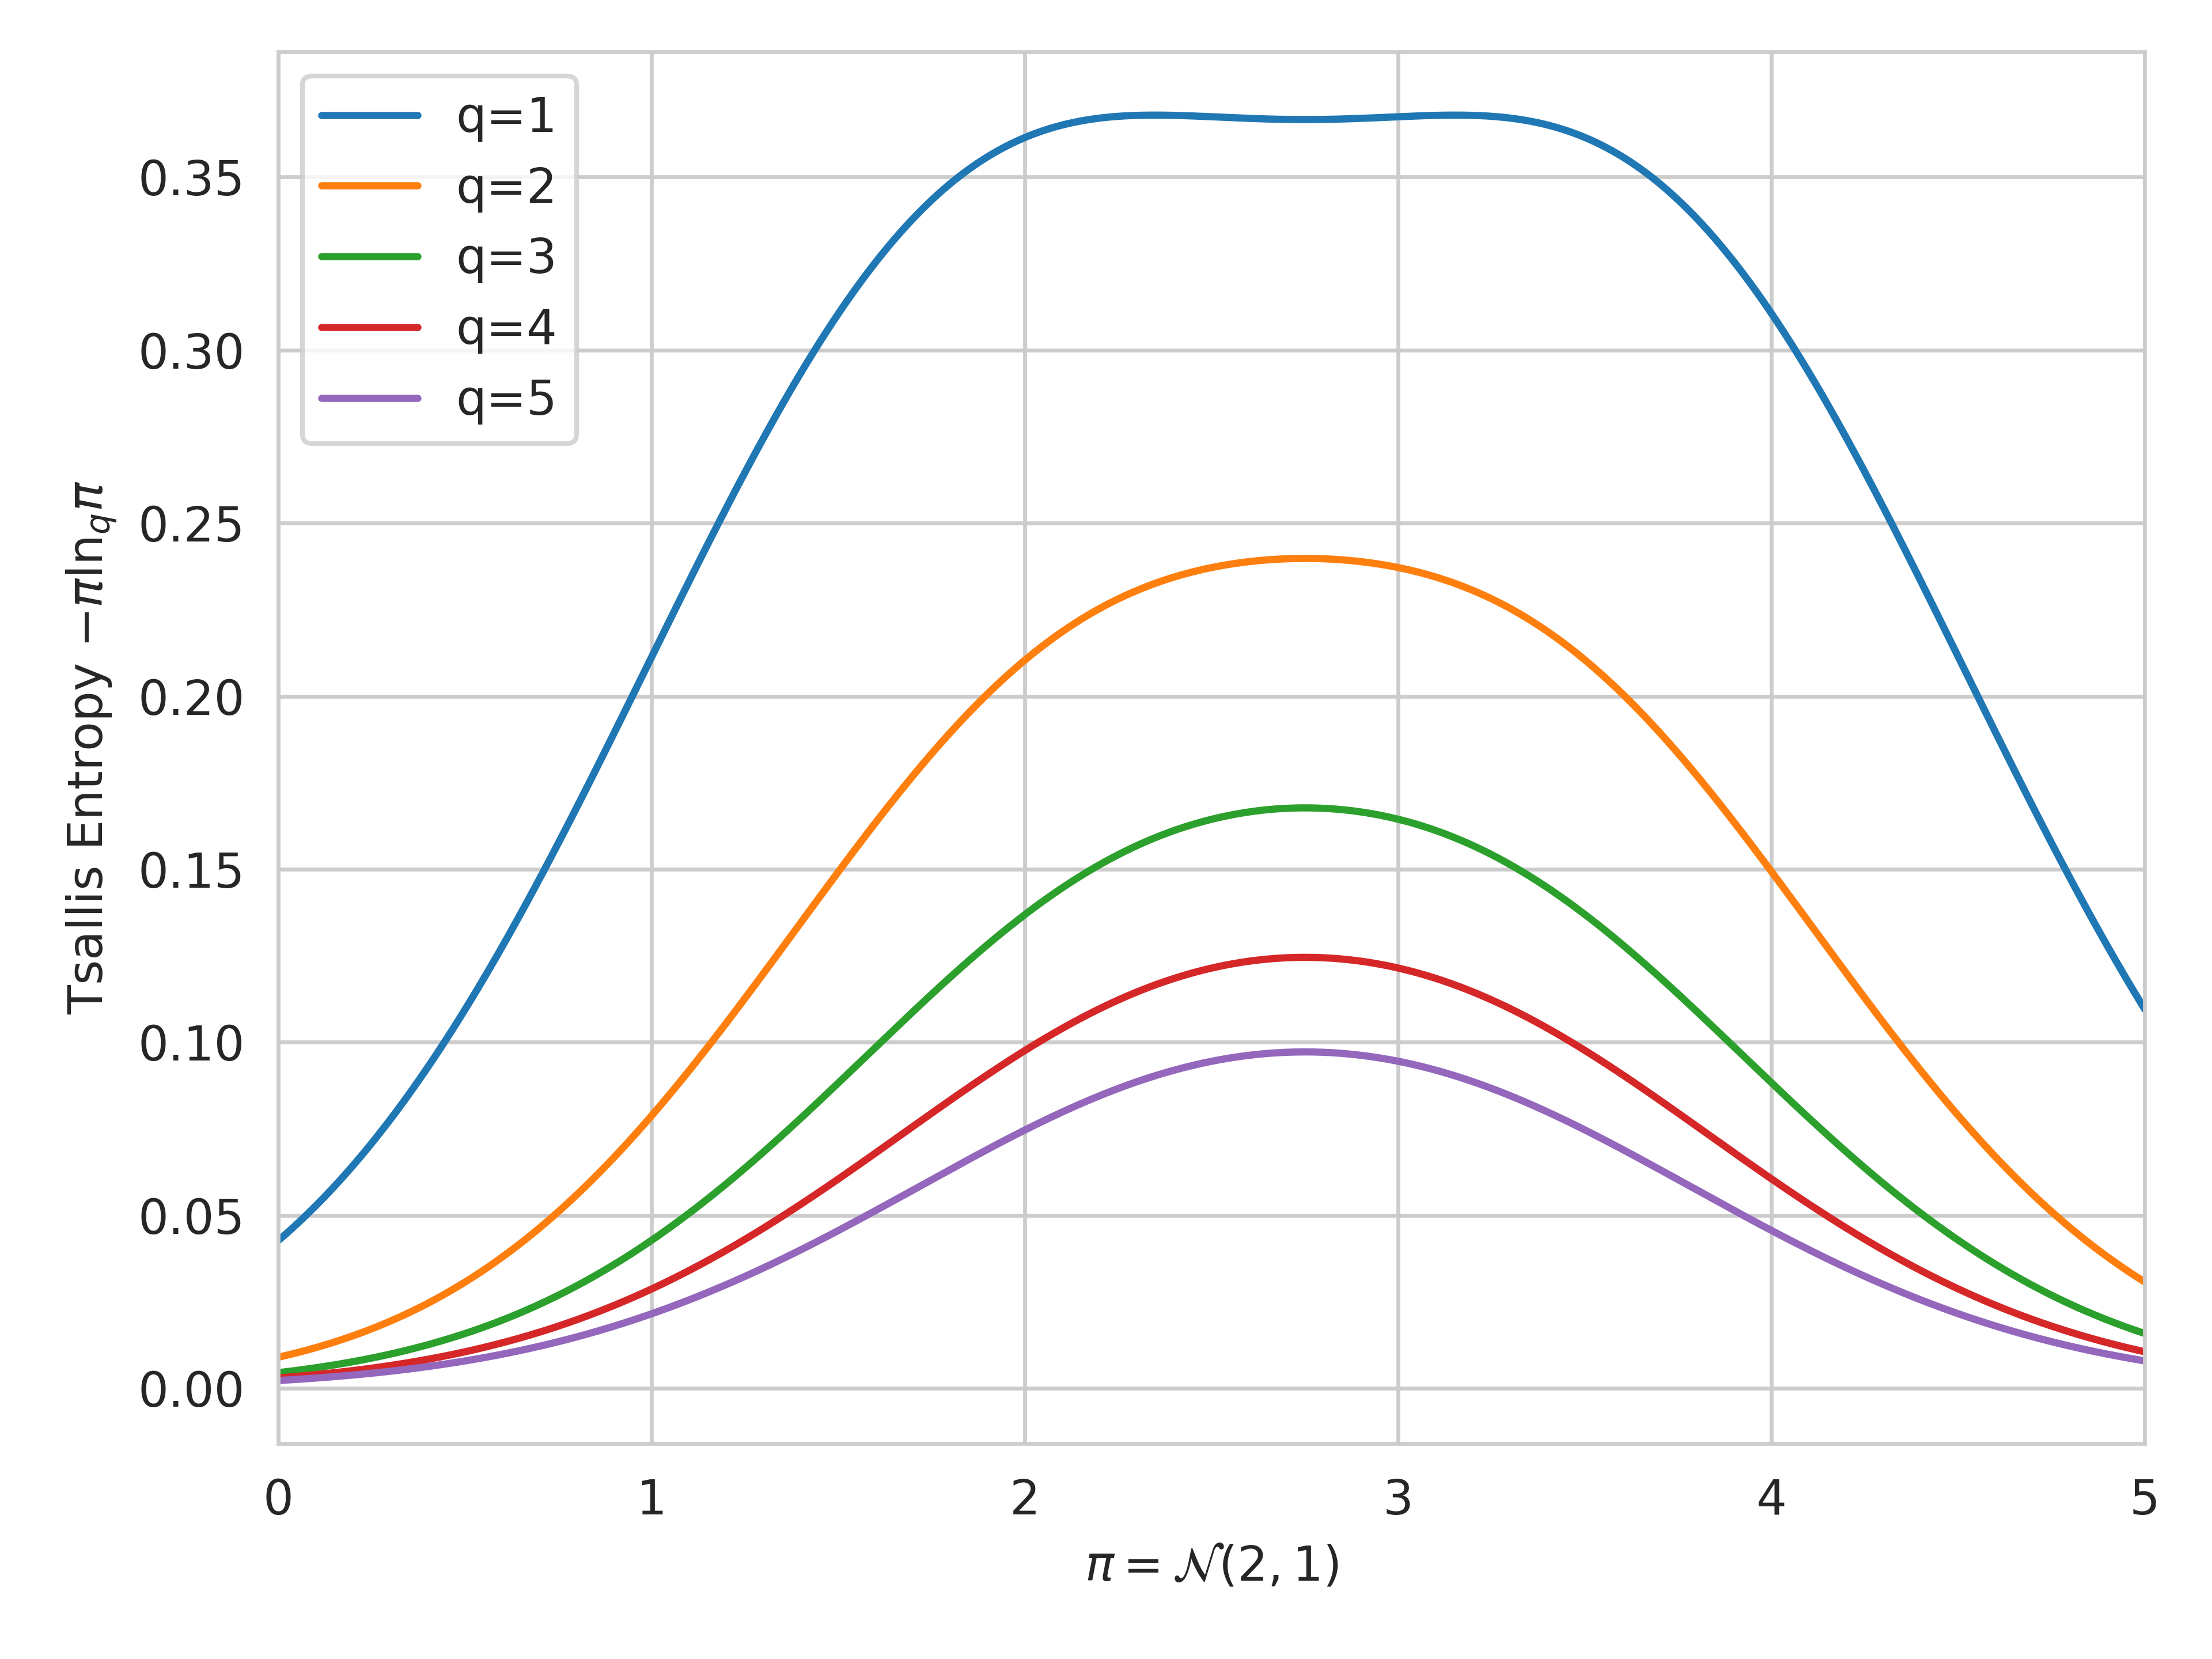
\includegraphics[width=\textwidth]{img/tsallis_entropy.png}
%         \label{fig:y equals x}
%     \end{subfigure}
%     \hfill
%     \begin{subfigure}[b]{0.49\textwidth}
%         \centering
%         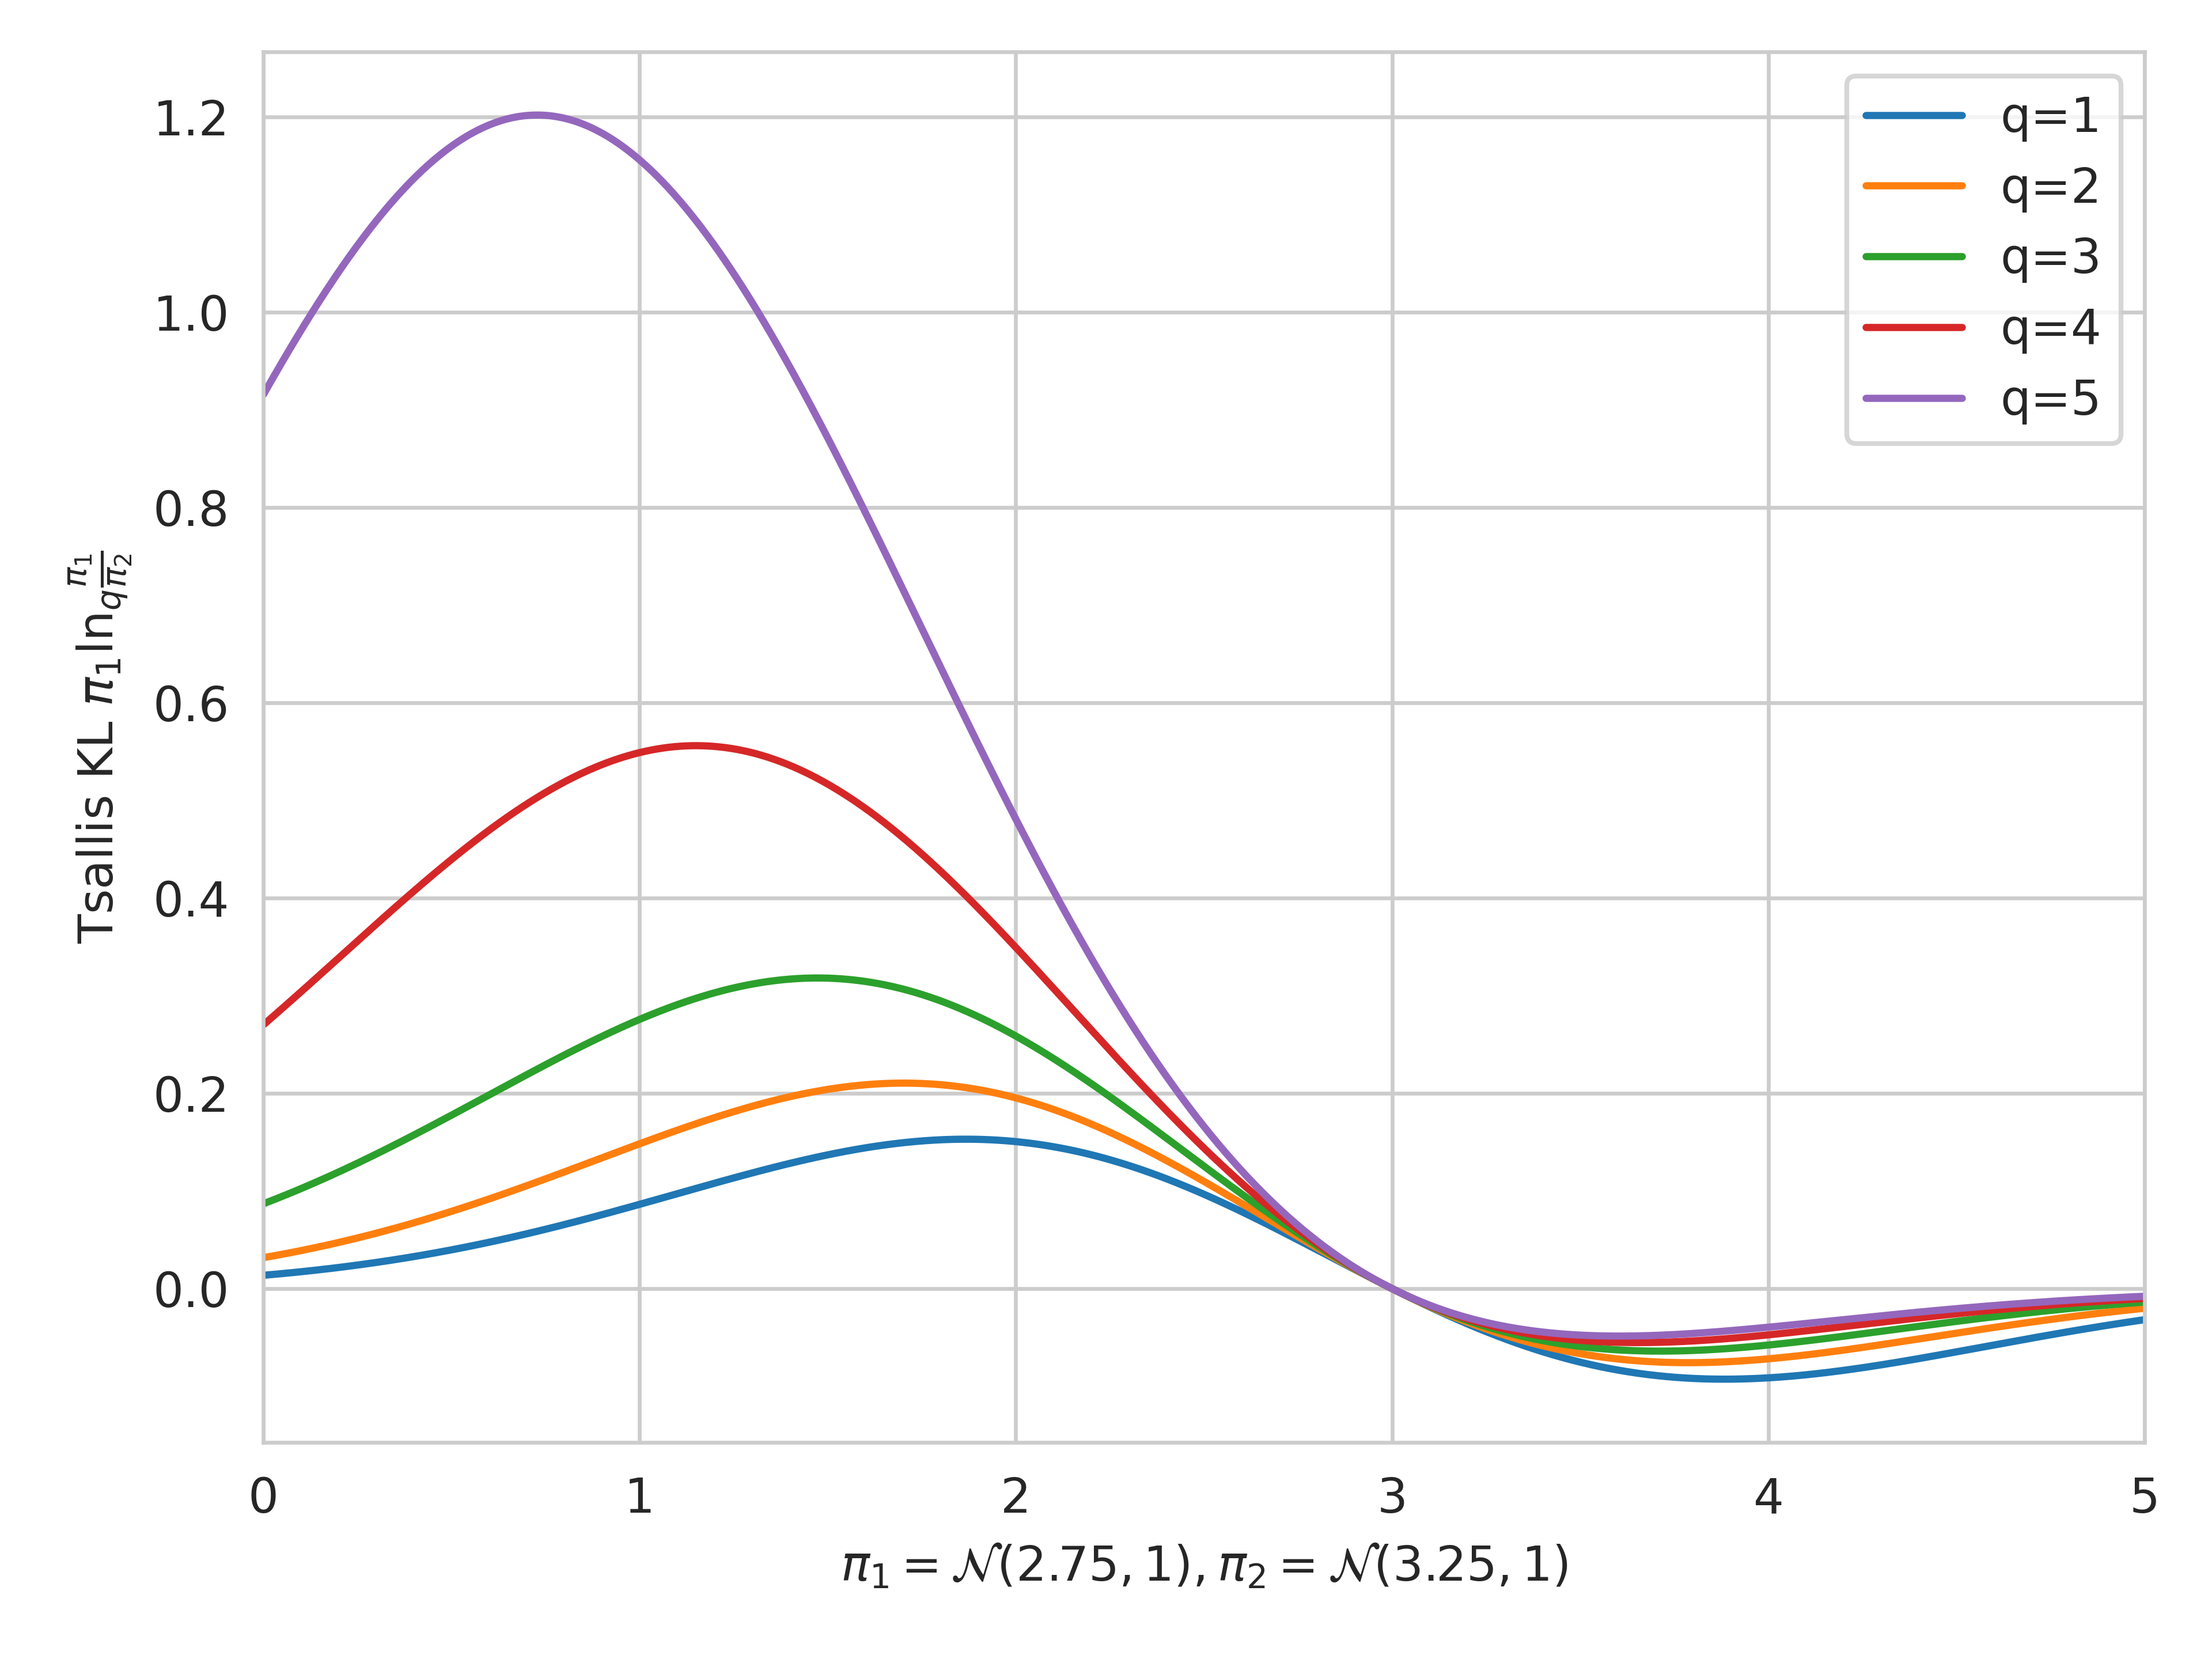
\includegraphics[width=\textwidth]{img/tsallis_kl.png}
%         \label{fig:three sin x}
%     \end{subfigure}
%     \caption{Estimation of policy ratio $\frac{\pi_{k+1}}{\pi_k}$ during learning of Munchausen DQN on \texttt{CartPole-v1} and \texttt{LunarLander-v2}.
%     Notice the $y$-axis is at the magnitude of $10^{35}$.
%     }
%     \label{fig:mdqn_policy_ratio}
% \end{figure}


Very recently \citet{zhu2023generalized} proposed in RL to exploit Tsallis KL divergence which generalizes Tsallis entropy.  
They proved that the regularized optimal policy takes a similar form to \eq{\ref{eq:average}}:
% Recall that, this definition is different from the statistical physics definition \citep{Furuichi2004-fundamentals-qKL}:
\begin{align}
    \begin{split}
        \qKLany{\pi}{\mu} = \AdaAngleProduct{\pi}{\logq{\frac{\pi}{\mu}}}, \quad \pi_{k+1} = \pi_{k} \exp_q\AdaBracket{\frac{Q_k}{\tau} - \psi\AdaBracket{\frac{Q_k}{\tau}} }.
    \end{split}
    \label{eq:tkl_policy}
\end{align}
\eq{\ref{eq:tkl_policy}} is important to our application of offline RL where we show the in-sample softmax becomes in-sample sparsemax.



\begin{figure}[t]
    \centering
    \begin{subfigure}[b]{0.245\textwidth}
        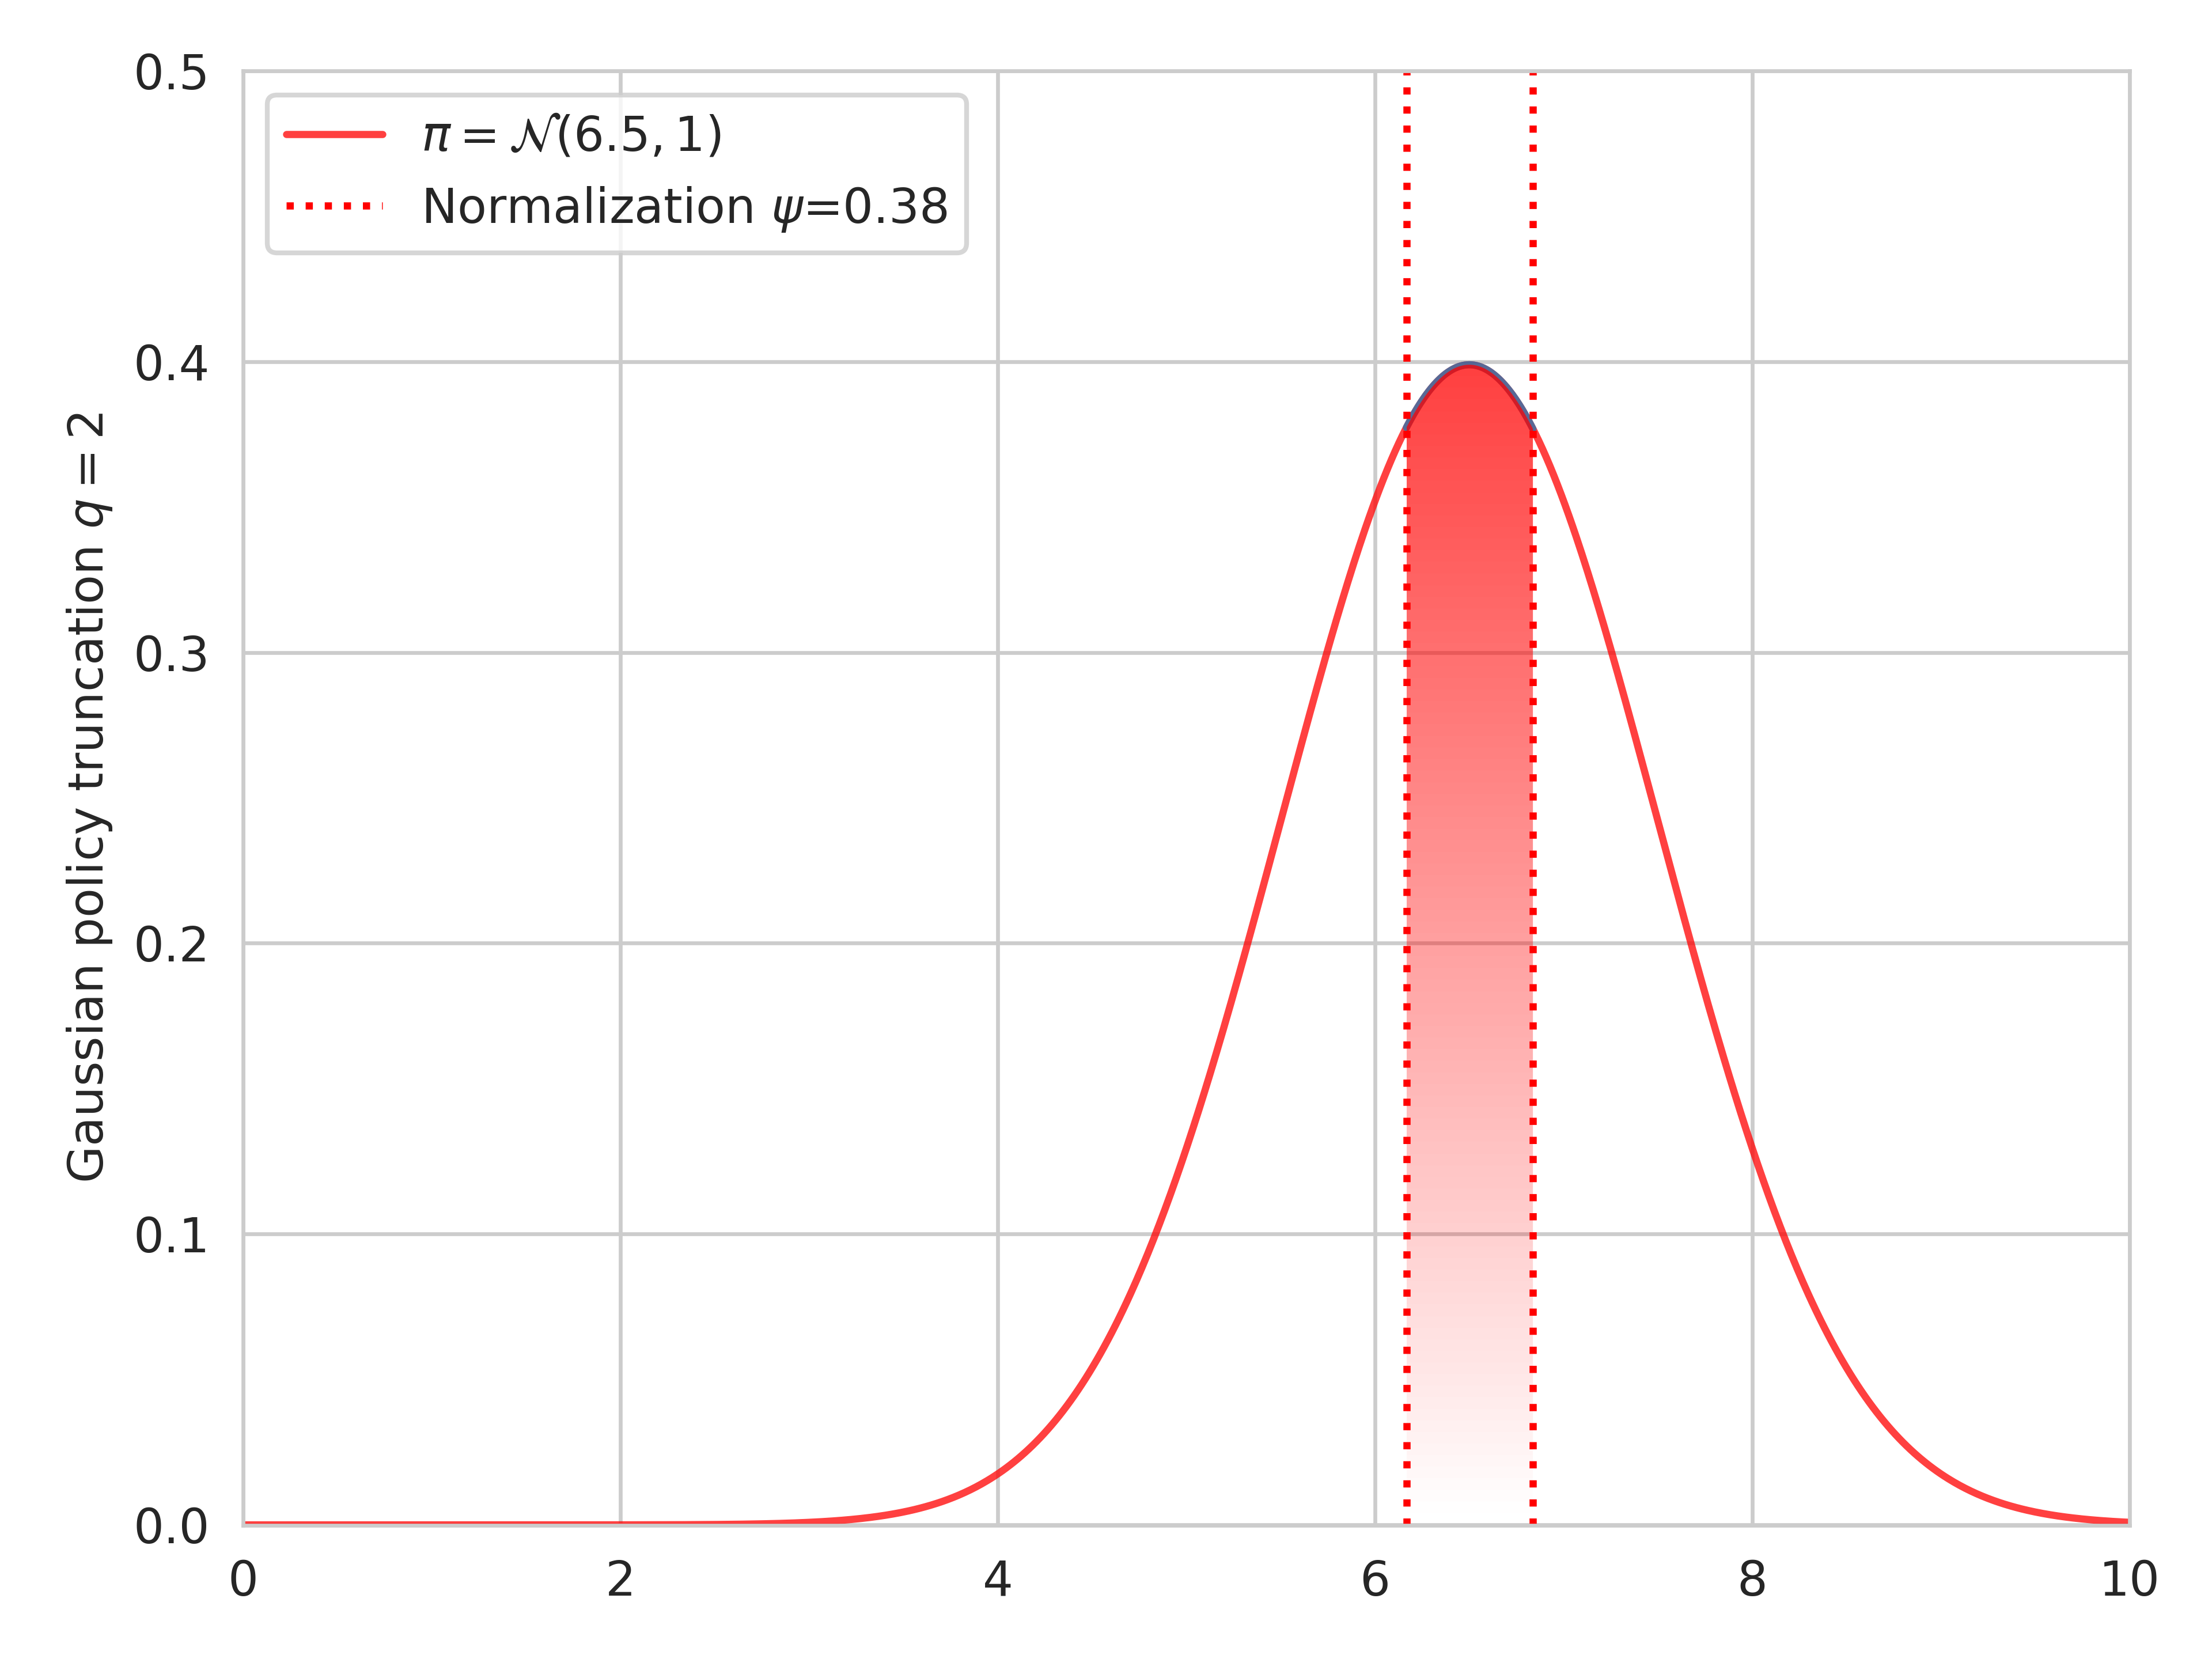
\includegraphics[width=\textwidth]{img/q2_Gaussian_sparsemax.png}
    \end{subfigure}
    \begin{subfigure}[b]{0.245\textwidth}
        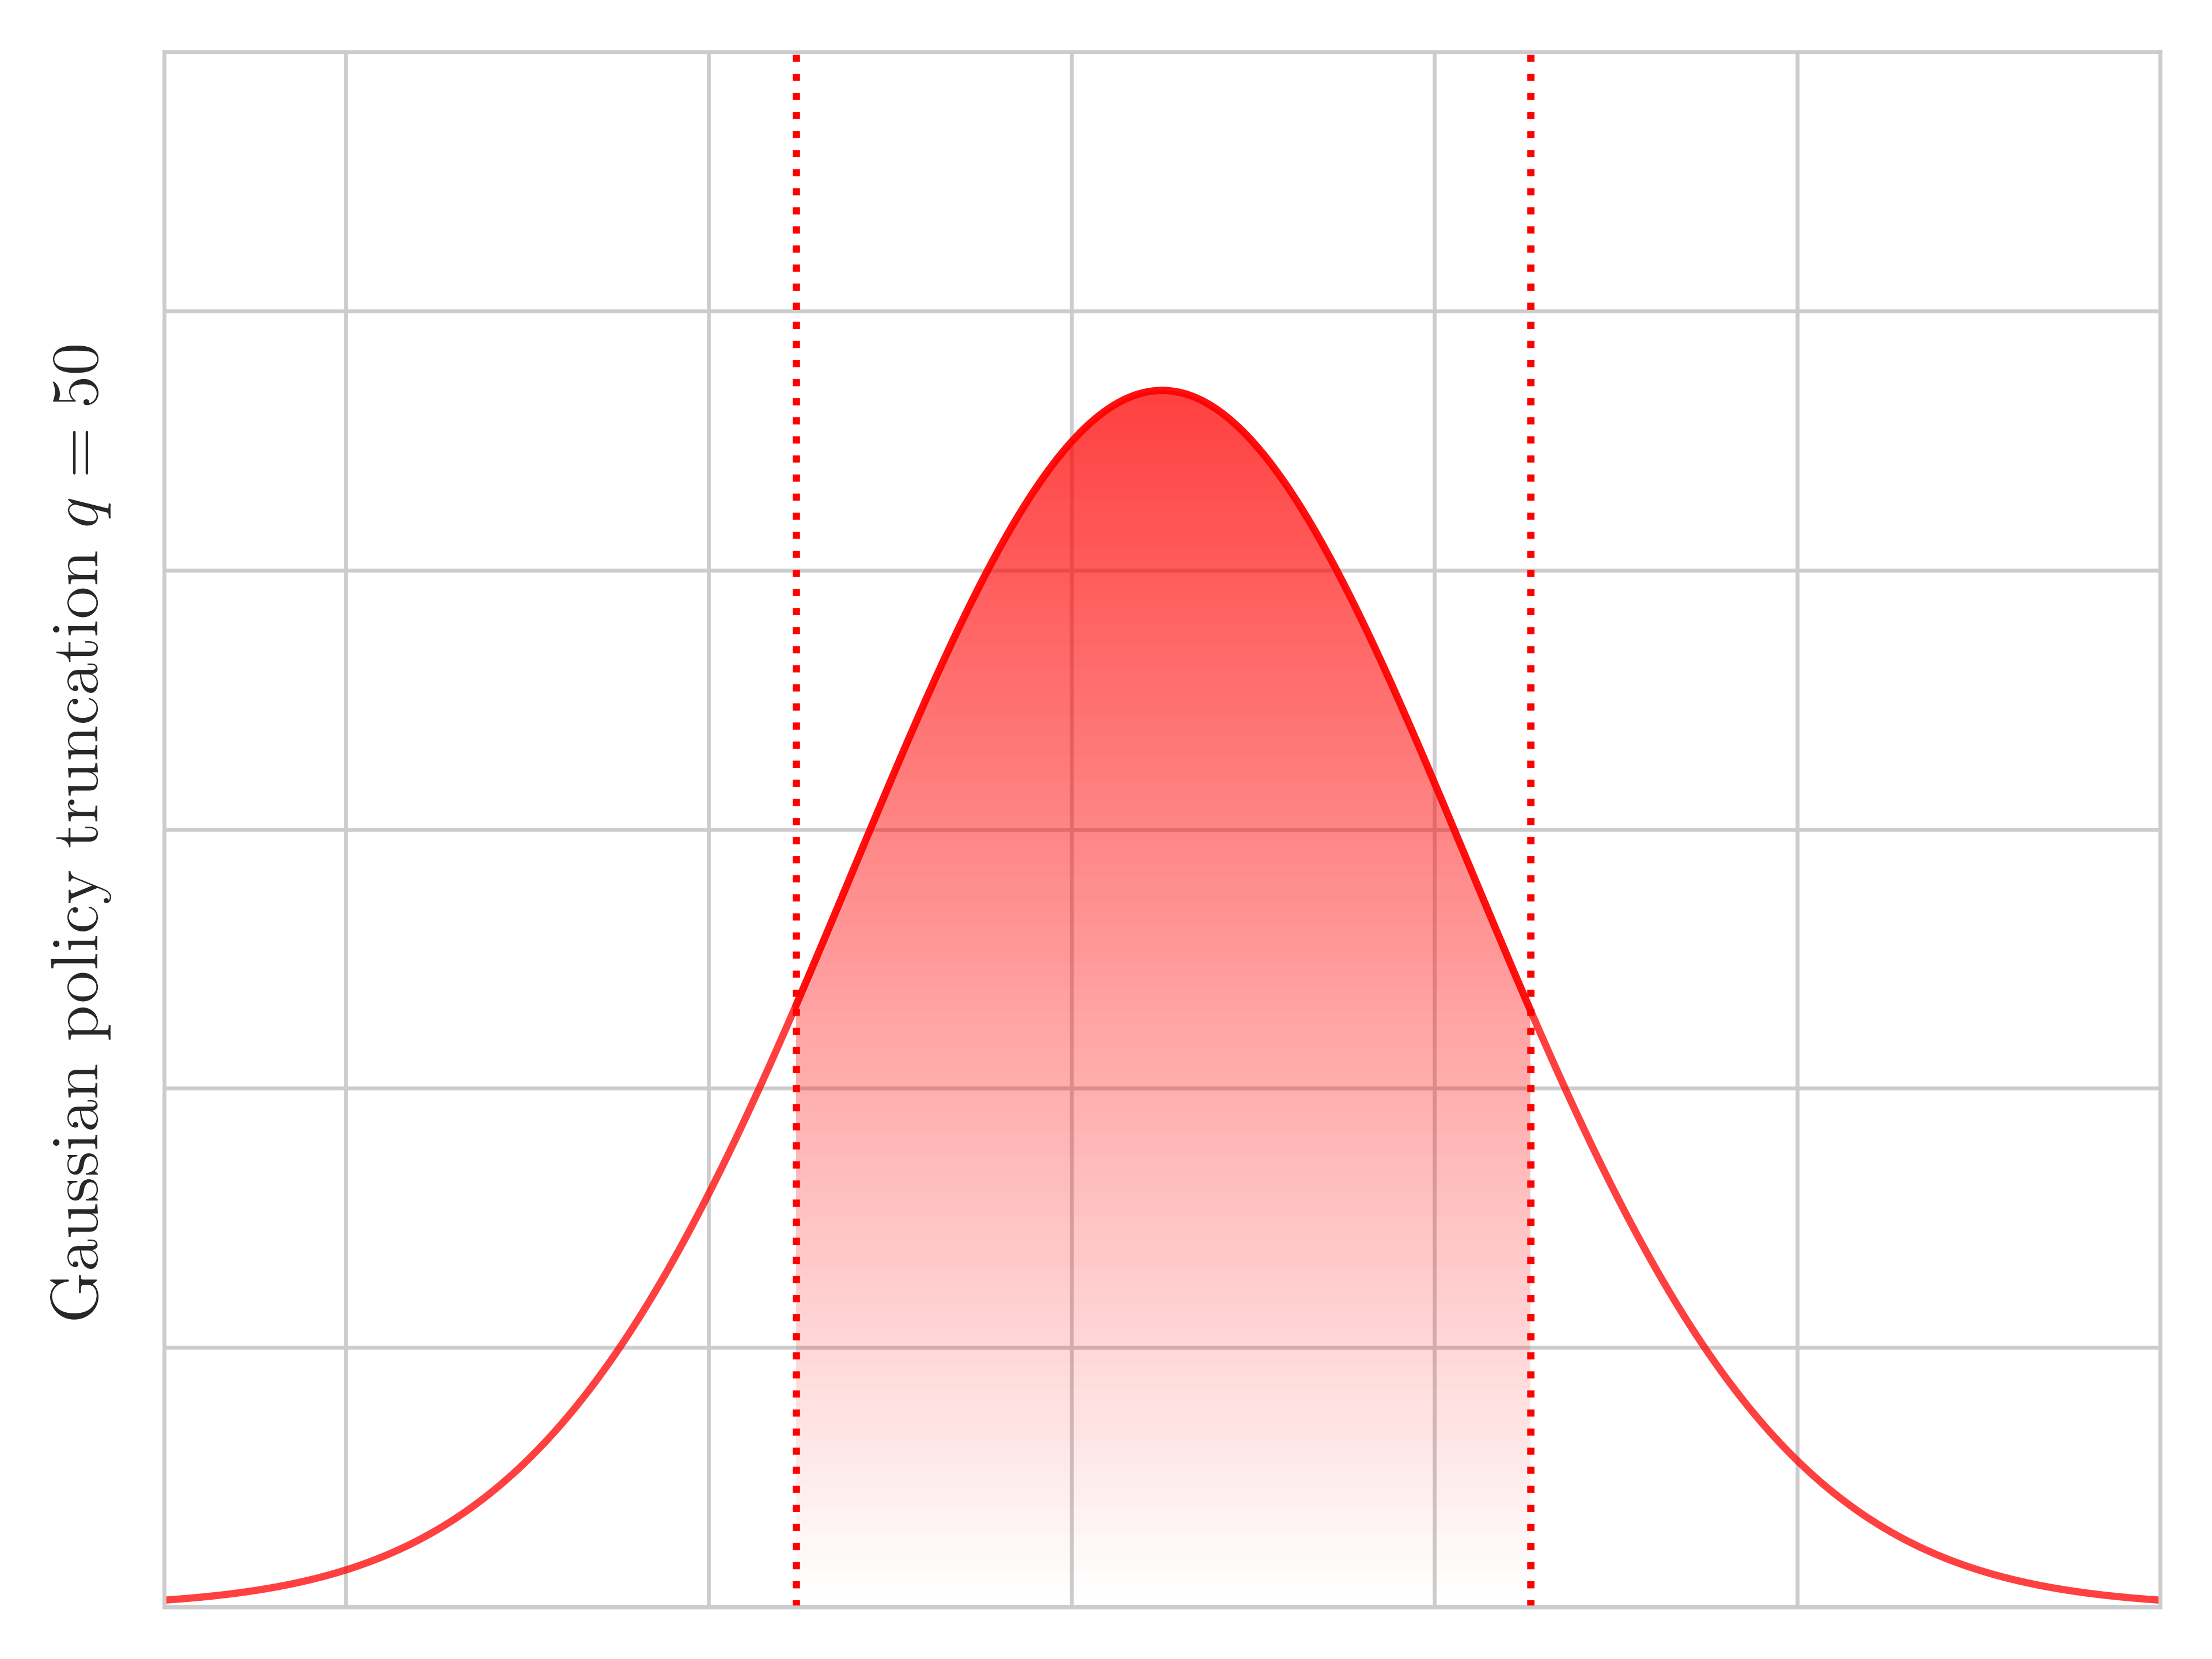
\includegraphics[width=\textwidth]{img/q50_scaled_Gaussian_sparsemax.png}
    \end{subfigure}
    \begin{subfigure}[b]{0.245\textwidth}
        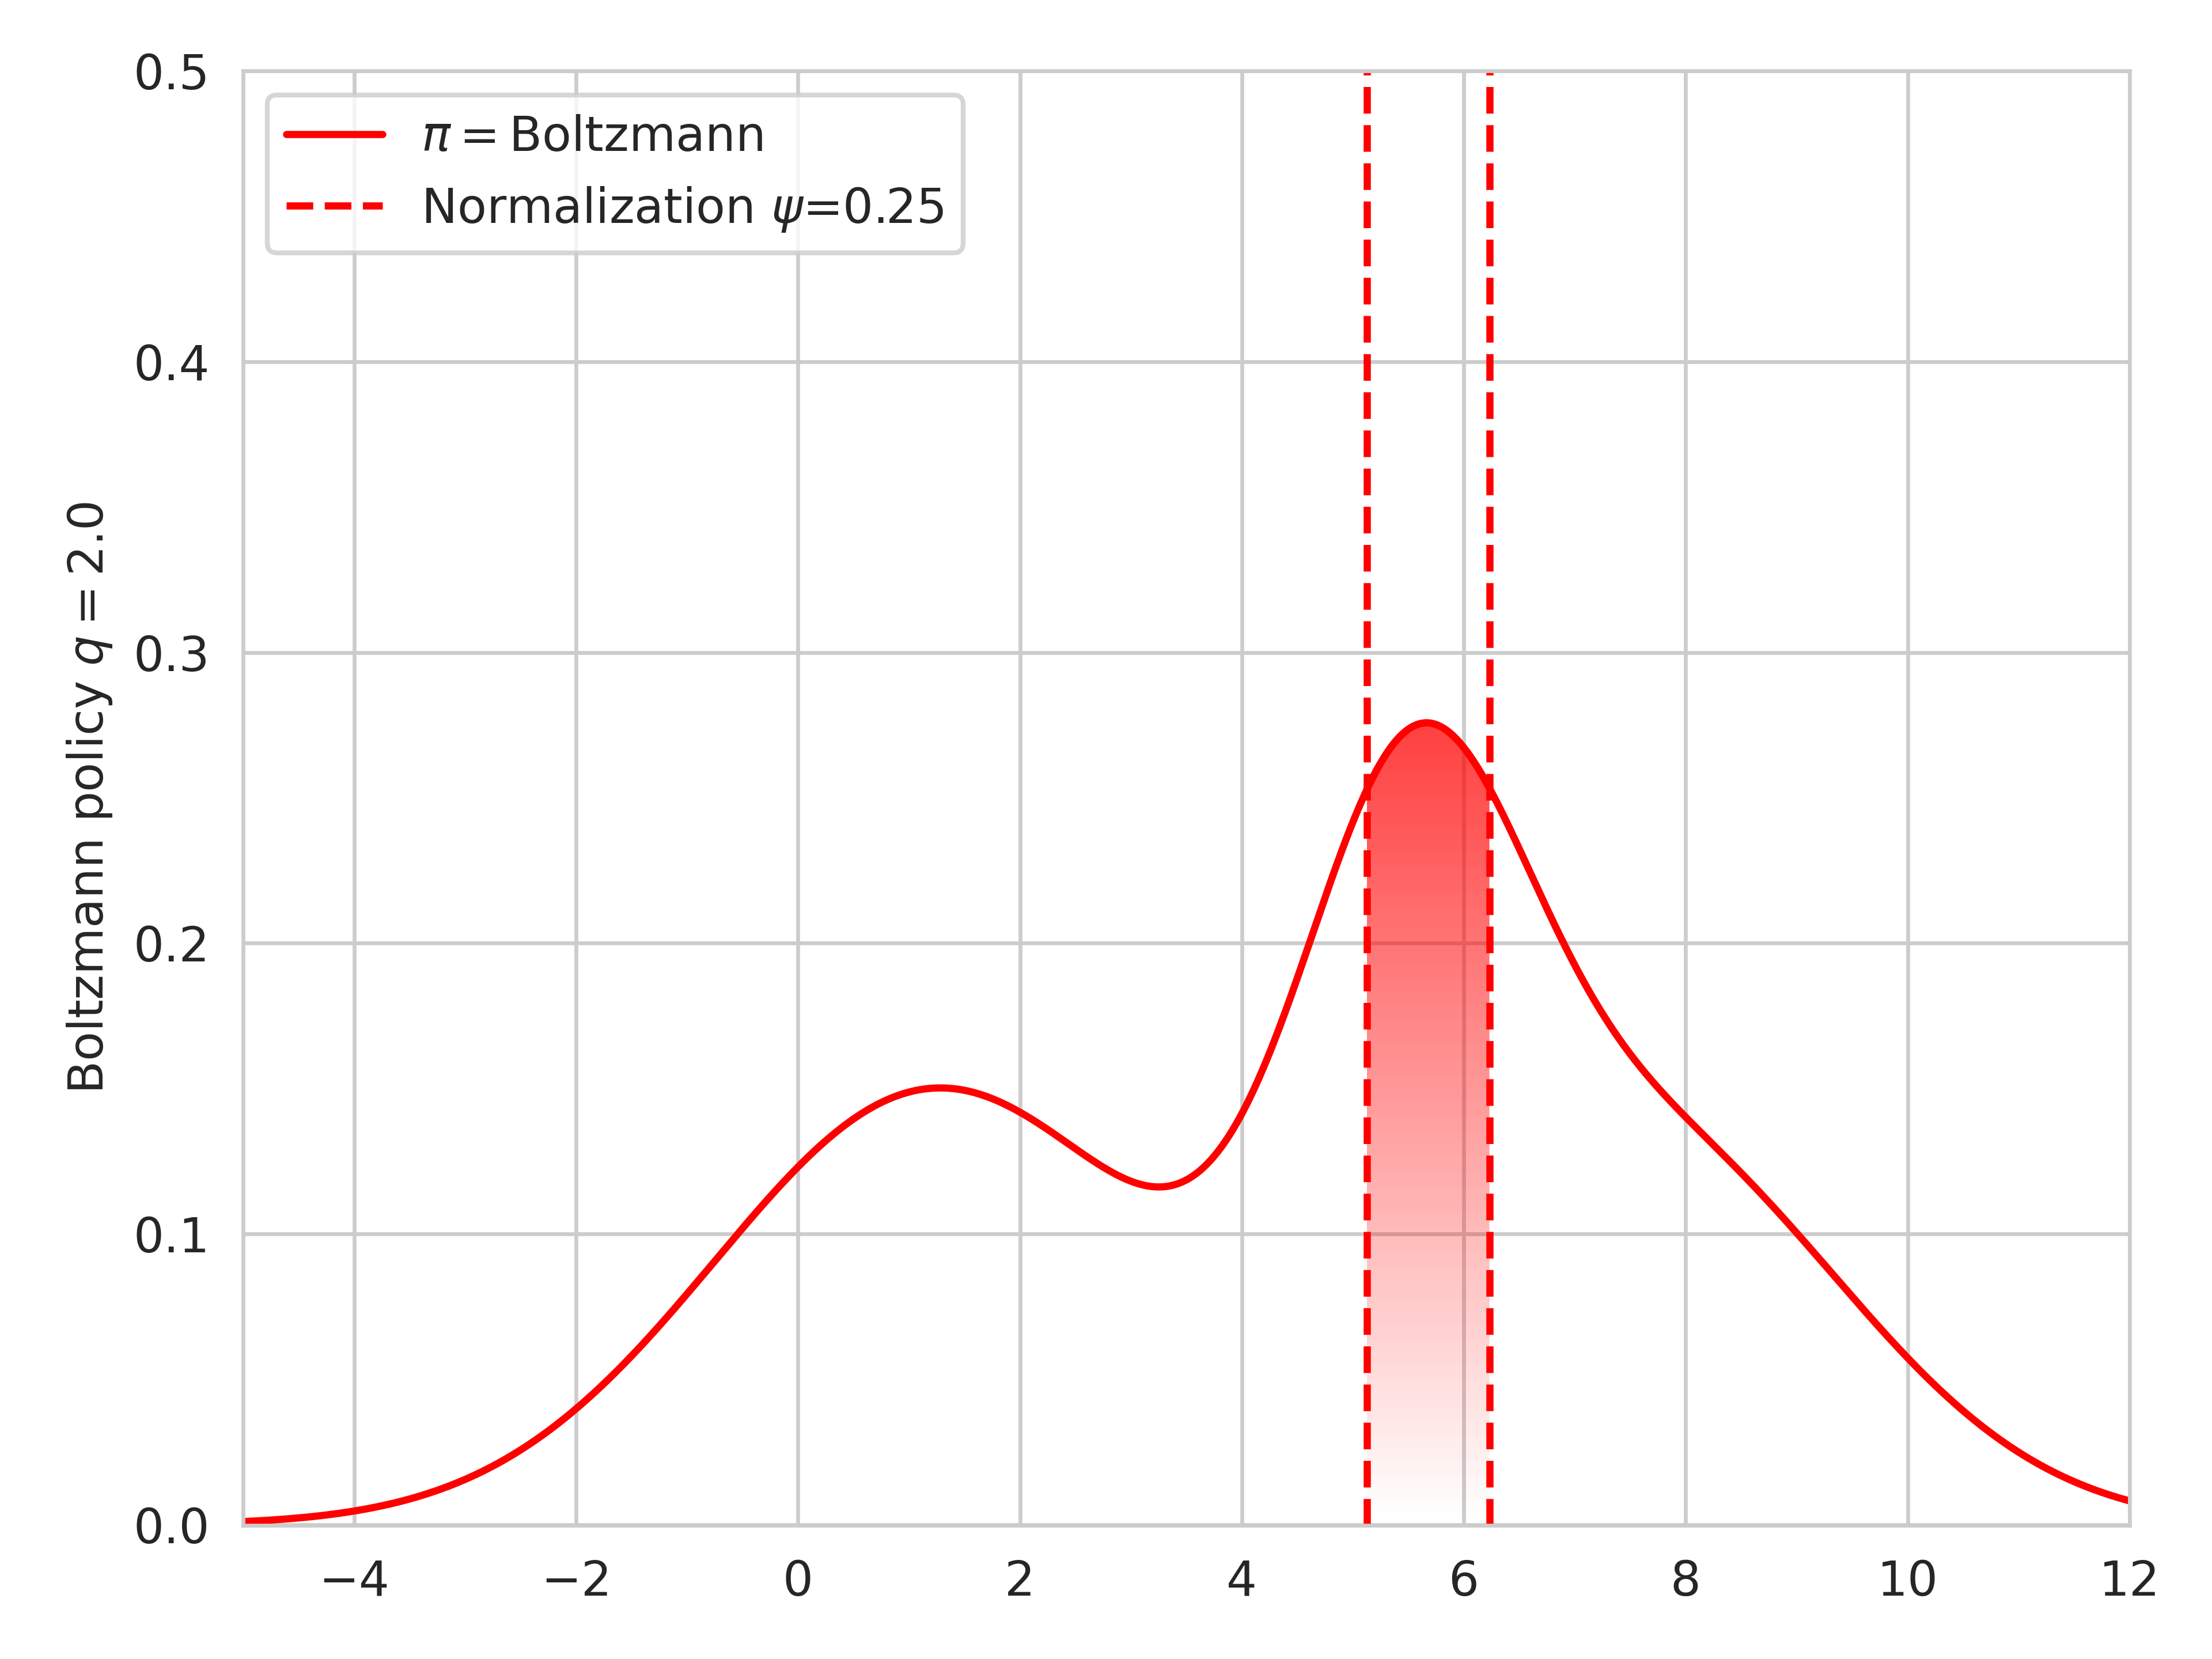
\includegraphics[width=\textwidth]{img/q2.0_Boltzmann_sparsemax.png}
    \end{subfigure}
    \begin{subfigure}[b]{0.245\textwidth}
        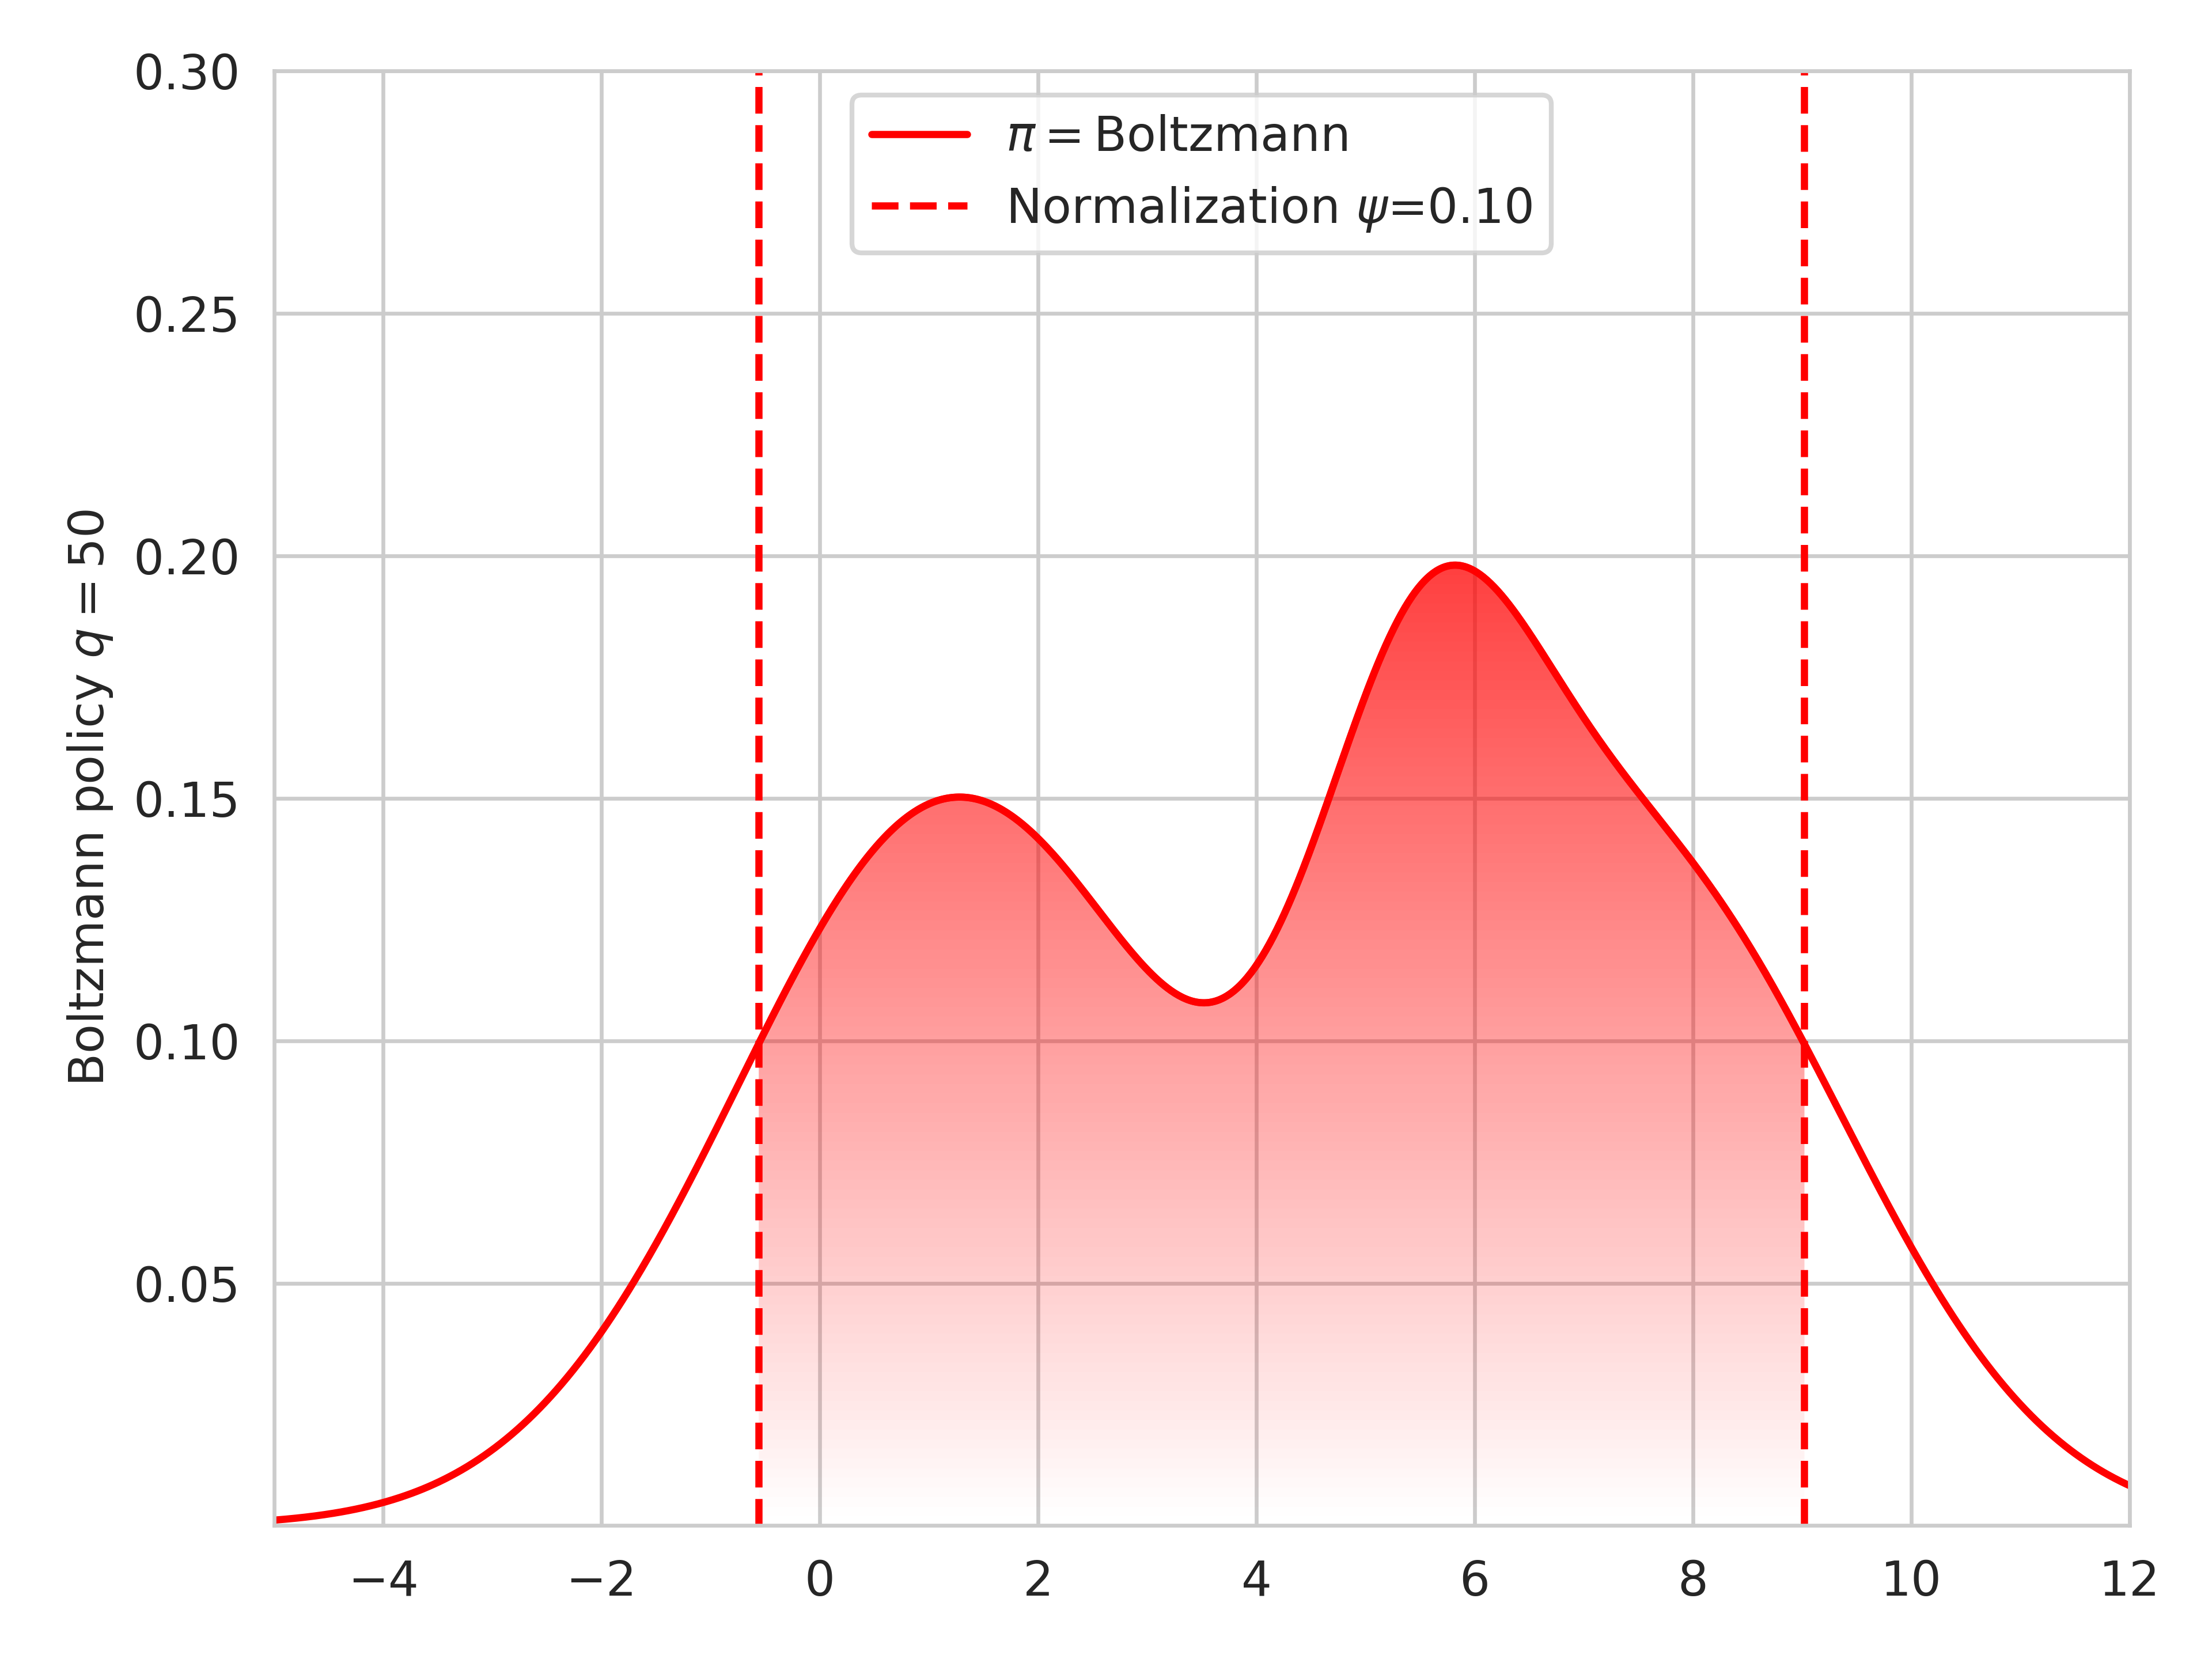
\includegraphics[width=\textwidth]{img/q50_Boltzmann_sparsemax.png}
    \end{subfigure}
    \caption{The sparsemax operator acting upon Gaussian and Boltzmann policies for $q=2$ and $q=50$ by truncating actions with values lower than $\psi$. 
    As $q\rightarrow \infty$ the policy tends toward uniform distribution.
    We assume the The dataset is generated by Tsallis policies such that the actions absent from the offline dataset are those being truncated.
    }
\end{figure}


\section{In-Sample Softmax for Offline RL}


To alleviate the out-of-distribution error, \citet{Fujimoto2019-InSampleMax} proposed the in-sample Bellman optimality equation to update only for actions present in the dataset:
\begin{align}
    \datasetOptimalQ = r + \gamma P_{*, \datasetPolicy} \datasetOptimalQ = r(s,a) + \gamma \expectation{s'\sim P(\cdot | s,a)}{\max_{a': \datasetPolicy(a'|s') > 0} \datasetOptimalQ(s',a')}.
    \label{eq:hardmax_offline}
\end{align}
Later, \citet{Xiao2023-InSampleSoftmax} proposed in-sample softmax to better estimate the policy inside the bracket since in the continuous case the hard max operator might be difficult to solve for.
By adding negative entropy regularization $\Omega(\pi) = \tau \entropy$ and imposing the data support constraint, the in-sample softmax Bellman optimality equation has the following evaluation step:
\begin{align}
    \datasetOptimalQ = r(s,a) +  \gamma \expectation{s'\sim P(\cdot | s,a)}{ \sum_{a': \datasetPolicy(a'|s') > 0} \!\!\!\!\! \pi(a'|s') \AdaBracket{\datasetOptimalQ(s',a') - \tau\entropy(\cdot|s')}}.
    \label{eq:insample_softmax}
\end{align}
By choosing the maximizer policy the above equation takes the form:
\begin{align}
    \datasetOptimalQ = r(s,a) +  \gamma \expectation{s'\sim P(\cdot | s,a)}{\tau \ln \!\!\!\!\!\sum_{a': \datasetPolicy(a'|s') > 0} \!\!\!\!\! \exp\AdaBracket{\tau^{-1} \datasetOptimalQ(s',a')}}.
\end{align}
As the dataset support constraint poses a challenge to implementation, \citet{Xiao2023-InSampleSoftmax} proposed to transform the summation into an expectation to avoid directly computing the constraint: 
\begin{align}
    \begin{split}
    \sum_{a': \datasetPolicy(a'|s') > 0} \!\!\!\!\!\!\exp\AdaBracket{\tau^{-1}\datasetOptimalQ (s',a')} &= \!\!\!\!\!\!\sum_{a': \datasetPolicy(a'|s') > 0} \frac{\datasetPolicy(a'|s')}{\datasetPolicy(a'|s')} \exp\AdaBracket{\tau^{-1}\datasetOptimalQ (s',a')} \\
    &= \expectation{a'\sim\datasetPolicy(\cdot | s')}{\exp\AdaBracket{\tau^{-1}\datasetOptimalQ (s',a') - \ln\datasetPolicy(a'|s')}}.
    \end{split}
\end{align}
The expectation is approximated by Monte-Carlo sampling actions from the dataset.
Since the term $\exp\AdaBracket{\tau^{-1}\datasetOptimalQ (s',a')}$ appears also in the regularized softmax policy, in-sample softmax updates the policy towards 
\begin{align}
    \pi_{\datasetPolicy, k+1} \propto  \datasetPolicy(a|s) \exp\AdaBracket{\frac{Q_{\datasetPolicy, k}(s,a)}{\tau} - \ln\hat{\pi}_{\mathcal{D}}(a|s)},
    \label{eq:inac_policy}
\end{align}
where $\hat{\pi}_{\mathcal{D}}$ inside the exponential function is learned to imitate the behavior policy to avoid $\pi_{\mathcal{D}} = 0$ leading to an unbounded log-policy.

We interpret \eq{\ref{eq:inac_policy}} from another perspective.
the in-sample softmax policy can be decomposed into two terms:
the first term $\datasetPolicy(a|s) \exp\AdaBracket{\frac{Q_{\datasetPolicy, k}(s,a)}{\tau} }$ acts as a KL-regularized policy with respect to the behavior policy (see \eq{\ref{eq:average}}); 
the second term $\exp\AdaBracket{-\ln\hat{\pi}_{\mathcal{D}}(a|s)}$ can be seen as induced by another regularization $\Omega(\pi) = -\AdaAngleProduct{\pi}{\ln{\hat{\pi}_{\mathcal{D}}}}$, the cross entropy between the in-sample softmax policy and the behavior policy.


\section{Forward-Backward Tsallis Learning for Offline RL}

Summary:
\begin{itemize}
    \item Forward: Tsallis sparsemax policies generate the dataset. This assumption is not very strong since Tsallis entropy generalizes Shannon entropy and the behavior policy class is sufficiently rich.
    \item Backward: learn the optimal policy with the modified Tsallis entropy regularization. The learned policy differs from the conventional sparsemax policies in that no thresholding is required.
\end{itemize}



The key to both in-sample max \cite{Fujimoto2019-InSampleMax} and in-sample softmax \cite{Xiao2023-InSampleSoftmax} is the dataset support constraint.
In this paper, we propose to exploit the properties of sparsemax policies to naturally satisfy this constraint.
In a nutshell, we assume the behavior policies are Tsallis sparsemax policies, and therefore the actions not present in the dataset are with low probability and are exactly these truncated actions.
For simplicity, suppose the dataset is generated by the Tsallis sparsemax policy:
\begin{align}
    \datasetPolicy(a|s) = \AdaRectBracket{\frac{Q_{\datasetPolicy}(s,a)}{\tau_\mathcal{D}} - \psi\AdaBracket{\frac{Q_{\datasetPolicy}(s, \cdot)}{\tau_\mathcal{D}}}}_{+},  \quad \sum_{a\in K_\mathcal{D}(s)} \pi_\mathcal{D}(a|s)= 1,
\end{align}
where $\tau_\mathcal{D}$ is a unknown coefficient and $K_\mathcal{D}(s)$ denotes the set of allowable actions.
Now let us inspect the Bellman equation for the behavior policy:
\begin{align}
    \begin{split}
    Q_{\datasetPolicy}(s,a) &= r(s,a) +  \gamma \expectation{s'\sim P(\cdot | s,a)}{ \sum_{a'} \datasetPolicy(a'|s') \AdaBracket{Q_{\datasetPolicy}(s',a') - \tau_{\mathcal{D}} S_2(\datasetPolicy)(\cdot|s')}}. \\ 
    &= r(s,a) +  \gamma \expectation{s'\sim P(\cdot | s,a)}{ \tau_{\mathcal{D}} \AdaBracket{ \sum_{a' \in K_{\mathcal{D}}(s')} \AdaBracket{\frac{Q_{\datasetPolicy}(s',a')}{\tau_{\mathcal{D}}}}^2 - \psi \AdaBracket{\frac{Q_{\datasetPolicy}(s', \cdot)}{\tau_{\mathcal{D}}}}^2 + 1 }}\\
    &= r(s,a) +  \gamma \expectation{s'\sim P(\cdot | s,a)}{ \tau_{\mathcal{D}} \AdaBracket{ \sum_{a': \datasetPolicy(a'|s') > 0} \AdaBracket{\frac{Q_{\datasetPolicy}(s',a')}{\tau_{\mathcal{D}}}}^2 - \psi \AdaBracket{\frac{Q_{\datasetPolicy}(s', \cdot)}{\tau_{\mathcal{D}}}}^2 + 1 }}.
    \label{eq:insample_sparsemax}
    \end{split}
\end{align}
Here, $\max_{\pi \in \Delta(\mathcal{A})}\pi(a|s)Q(s,a) + \tau S_2(\pi(\cdot|s)) $ attains its maximum at $V(s) = \tau \sum_{a \in K(s)}\AdaBracket{ \frac{Q(s,a)}{\tau} }^2 - \psi\AdaBracket{\frac{Q(s, \cdot)}{\tau}}^2 + \tau$ \cite{Lee2018-TsallisRAL,Martins16-sparsemax}.
It is also possible to assume that $\datasetPolicy(a|s) = \exp_q\AdaBracket{\frac{Q_{\datasetPolicy}(s,a)}{\tau_\mathcal{D}} - \tilde{\psi}\AdaBracket{\frac{Q_{\datasetPolicy}(s, \cdot)}{\tau_\mathcal{D}}}}$ for general $q>2$, though in these cases the policy does not have a closed-form expression we have to resort to approximation.
Under the Tsallis behavior policy assumption, the dataset support constraint $a: \datasetPolicy(a|s) > 0$ coincides with the condition $a \in K_{\mathcal{D}}(s)$.
Moreover, the assumption actually assumes a forward process of learning a set of allowable actions $K_\mathcal{D}(s)$ given $Q_{\datasetPolicy}(s,a), \forall s,a$;
 and it naturally raises the possibility of \emph{backward Tsallis learning}: given the set of allowable actions $K_\mathcal{D}(s)$, learn an optimal policy that resembles $\datasetPolicy$ in the sense of $\pi_* \preceq \datasetPolicy$, i.e. putting probability mass only on the actions in $K_\mathcal{D}$.

 The backward Tsallis learning consists in learning $\pi_{t, \datasetPolicy} \preceq \datasetPolicy$ given $K_\mathcal{D}$.
% However, it should be noted that the learned policy no longer requires a thresholding function $\tilde{\psi}$ since the set of allowable actions $K_\mathcal{D}$ is given, hence no action need to be explicitly truncated.
% Specifically, we propose to modify the learned policy form as 
\begin{align}
    \pi_{t+1, \datasetPolicy}(a|s) = \exp_q\AdaBracket{\frac{Q_{t, \datasetPolicy}(s,a)}{\tau} - \tilde{\psi}{\AdaBracket{\frac{Q_{t, \datasetPolicy}(s,\cdot)}{\tau}}}},  \quad \sum_{a\in K_{\mathcal{D}}(s)} \pi_{t+1, \datasetPolicy} = 1.
    \label{eq:proposal_policy}
\end{align}
When $q=2$, the policy is a variant of categorical distributions, which is less susceptible to numerical issues than exponential functions \cite{Tsai2021-selfsupervisedRelativePredictiveCoding}.



% That is, the backward Bellman optimality equation becomes:
% \begin{align}
%     \begin{split}
%         \datasetOptimalQ(s,a) &= r(s,a) +  \gamma \expectation{s'\sim P(\cdot | s,a)}{ \sum_{a' \in K_\mathcal{D}(s')} \pi_{*, \datasetPolicy}(a'|s') \AdaBracket{\datasetOptimalQ(s',a') - \tau S_2(\pi_{*, \datasetPolicy})(\cdot|s')}}. 
%     \end{split}
% \end{align}
% The term inside the expectation is now:
% \begin{align}
%     \begin{split}
%         & \sum_{a' \in K_\mathcal{D}(s')} \pi_{*, \datasetPolicy}(a'|s') \AdaBracket{\datasetOptimalQ(s',a') - \tau S_2(\pi_{*, \datasetPolicy})(\cdot|s')} \\ 
%          &= \sum_{a' \in K_\mathcal{D}(s')} \pi_{*, \datasetPolicy}(a'|s') \AdaBracket{ \datasetOptimalQ(s',a') + \frac{\tau}{2}(1 - \pi_{*, \datasetPolicy}(a'|s')) } \\
%          &= \sum_{a' \in K_\mathcal{D}(s')} \pi_{*, \datasetPolicy}(a'|s') \AdaBracket{ \datasetOptimalQ(s',a') - \frac{\tau}{2}\pi_{*, \datasetPolicy}(a'|s') } + \frac{\tau}{2} \\
%          &= \sum_{a' \in K_\mathcal{D}(s')} \frac{\AdaRectBracket{ \tau^{-1}Q_{t, \datasetPolicy}(s,a)}_+ }{\sum_{b\in K_\mathcal{D}(s')}\tau^{-1} Q_{t, \datasetPolicy}(s,b)}
%     \end{split}
% \end{align}


\textbf{Why use Tsallis backward learning? }
If the Tsallis dataset policy assumption holds, and Tsallis backward learning is adopted, 
then the KL divergence between the learned policy and the behavior policy can be bounded as:
\begin{align}
    \begin{split}
        &\KLany{\pi_t(\cdot|s)}{\datasetPolicy(\cdot|s)} = \expectation{a\sim\pi_{t}(\cdot | s)}{\ln \pi_{t}(a|s) - \ln\datasetPolicy(a|s)} \\
        & = \expectation{a\sim\pi_{t}(\cdot | s)}{\underbrace{\ln \pi_{t}(a|s) - \ln_q\pi_{t}(a|s)}_{(1)} + \underbrace{\ln_q\pi_{t}(a|s) -  \ln\datasetPolicy(a|s)}_{(2)} + \underbrace{\ln_q\datasetPolicy(a|s) - \ln\datasetPolicy(a|s)}_{(3)} } .
    \end{split}
\end{align}
Let us now respectively bound the three terms:
\begin{align}
    \begin{split}
        (1): &\ln \pi_{t}(a|s) - \ln_q\pi_{t}(a|s) = (q-1) \AdaRectBracket{\frac{d}{dq}\ln_q \pi_t(a|s) + \ln_q\pi_t(a|s)\ln\pi_t(a|s)}\\
        &= (q-1)\AdaRectBracket{\pi_t^{q-1}(a|s)\ln\pi_t(a|s) - \frac{\pi_{t}^{q-1}(a|s)-1}{(q-1)^2} + \ln_q\pi_t(a|s)\ln\pi_t(a|s)}\\
        &= (q-1)\pi_{t}^{q-1}(a|s)\ln\pi_t(a|s) - \ln_q\pi_t(a|s) + (q-1)\ln_q\pi_t(a|s)\ln\pi_t(a|s)\\
        % &= (q-1)\pi_{t}^{q-1}(a|s)\ln\pi_t(a|s) - \AdaBracket{ \frac{Q_{t-1}(s,a)}{\tau} - \tilde{\psi}\AdaBracket{\frac{Q_{t-1}(s,\cdot)}{\tau}}}  + \ln\pi_t(a|s) \AdaBracket{ \frac{Q_{t-1}(s,a)}{\tau} - \tilde{\psi}\AdaBracket{\frac{Q_{t-1}(s,\cdot)}{\tau}}}
        & \leq (q-1)\pi_{t}^{q-1}(a|s)\ln\pi_t(a|s) + \frac{1}{q-1} - \ln\pi_t (a|s)\\
        &=  \AdaBracket{ (q-1)\pi_{t}^{q-1}(a|s) - 1}\ln\pi_t(a|s) + \frac{1}{q-1},
    \end{split}
\end{align}
where we leveraged the fact that $-\frac{1}{q-1} < \frac{Q_{t-1}(s,a)}{\tau} - \tilde{\psi}\AdaBracket{\frac{Q_{t-1}(s,\cdot)}{\tau}} < 0, \, \forall a\in K(s)$. If $a \notin K_{\mathcal{D}}(s)$, then $\ln\pi_t(a|s) = -\infty$ and the KL term is unbounded.
We repeat the same trick to yield an upper bound $\AdaBracket{ (q-1)\datasetPolicy^{q-1}(a|s) - 1}\ln\datasetPolicy(a|s) + \frac{1}{q-1}$  for (3); and and upper bound $\frac{1}{q-1}$  for (2).

As a summary, we can state for $q>1$ that:
\begin{align}
    \begin{split}
    &\KLany{\pi_t(\cdot|s)}{\datasetPolicy(\cdot|s)}  \leq  \\
    &\quad K_{\mathcal{D}}(s){\AdaRectBracket{\AdaBracket{ (q-1) \datasetPolicy^{q-1}(a|s) - 1}\ln\datasetPolicy(a|s) + \AdaBracket{  (q-1) \pi_{t}^{q-1}(a|s) - 1}\ln\pi_t(a|s) + \frac{3}{q-1}}}.
\end{split}
\end{align}
This result suggests that in order to keep the learned policy close to the behavior policy, one should choose $q$ such that $(q-1)\pi^{q-1}_t(a|s)$ close to 1.

\textbf{Difference with In-sample Softmax. }
Our proposal is seemingly similar to in-sample softmax \cite{Xiao2023-InSampleSoftmax}.
However, the two methods are radically different: in-sample softmax requires satisfying the dataset support constraint during learning to alleviate the out-of-distribution error, and is motivated by the observation that taking softmax is easier than the hard max operator \eq{\ref{eq:hardmax_offline}}.
On the other hand, we assume the behavior policies are Tsallis policies and as such the actions not present in the dataset are those being truncated.
This viewpoint leads to the natural satisfaction of the dataset support constraint.

Furthermore, the assumption naturally leads to the choice of Tsallis regularized backward learning which recovers in-sample softmax as a special case when $q=1$.
Since softmax policies have full support, there always exists non-negligible probabilities for suboptimal actions; while for \eq{\ref{eq:proposal_policy}} the optimal policy can switch between greedy policy when $Q_{t, \datasetPolicy}(s,a) \leq 0, \forall a\neq a^*$ and multimodal policy when some actions have positive values.

\begin{remark}
    Tsallis entropy regularization has not been popular since its proposal in RL \cite{Lee2018-TsallisRAL}.
    One of the main reasons is the sparsemax policies are not suitable for online RL since the exploration is handicapped resulted from the action truncation.
    However, in offline RL this drawback vanishes, and theoretically it provides a better in-sample algorithm that the constraint is satisfied implicitly. 
\end{remark}


\section{Implementation}

Let $\theta, \phi, \omega$ denote the parametrization of networks for $Q$, $\pi_{\datasetPolicy}, \datasetPolicy$, respectively.
In-sample softmax updates the policy towards 
\begin{align}
    \pi_{\datasetPolicy, Q_{\theta}}(a|s) = \datasetPolicy(a|s)\exp\AdaBracket{\frac{Q_{\theta}(s,a) - Z(s)}{\tau} - \ln \pi_{\omega}(a|s)},
    \label{eq:insample_policy}
\end{align}
where $Z(s)$ denotes the normalization constant and is necessary since the policy is updated by minimizing KL divergence:
\begin{align*}
    &\KLany{\pi_{\datasetPolicy, Q_{\theta}}(\cdot|s)}{\pi_{\phi}(\cdot | s)} = \expectation{a \sim \pi_{\datasetPolicy, Q_{\theta}}(\cdot|s) }{\ln \pi_{\datasetPolicy, Q_{\theta}}(a|s) - \ln \pi_{\phi}(a | s)} \\
    &= \expectation{a \sim \datasetPolicy(\cdot|s)}{ - \exp\AdaBracket{\frac{Q_{\theta}(s,a) - Z(s)}{\tau} - \ln \pi_{\omega}(a|s)} \ln\pi_{\phi}(a|s) },
\end{align*} 
where the $\datasetPolicy$ term in $ \pi_{\datasetPolicy, Q_{\theta}}$ is absorbed into the expectation, so the KL divergence loss can be minimized by sampling actions from the offline dataset.

We follow the same setup here, but replacing every appearance of $\ln, \exp$ to their \qlog and $q$-exponential counterpart.
In practice, computing the thresholding function $\psi$ requires sorting in the discrete control setting and it remains unclear how to accurately estimate it for the continuous control problems.
We found it improves the performance by simply removing $\psi$ and renormalize the policy.
In this case, thresholding can still be achieved by simply learning $Q_{\theta} \rightarrow 0$.
That is, the learned policy form becomes $\pi_{t+1}(a|s) \propto \AdaRectBracket{Q_{\theta}(s,a)}_{+}$.
In order to also sample actions from the dataset when updating the policy, we repeat the derivation in \eq{\ref{eq:insample_policy}} but for the sparsemax policy.
% Let us define $q_{\theta}(s,a) := \frac{Q_{\datasetPolicy, k}(s,a)}{\tau} - \psi\AdaBracket{\frac{Q_{\datasetPolicy, k}(s,\cdot)}{\tau}}$ for convenience:
\begin{align}
    \begin{split}
        \pi_{\datasetPolicy, k+1} (a|s) &= \datasetPolicy(a|s) \datasetPolicy(a|s)^{-1} \exp_q{Q_{\theta}(s,a)} \\
        &= \datasetPolicy(a|s)  \exp_q{\AdaBracket{\ln_2{\frac{1}{\datasetPolicy(a|s)}}}} \exp_q{Q_{\theta}(s,a)}\\
        &=  \datasetPolicy(a|s) \AdaBracket{ \exp_q\AdaBracket{Q_{\theta}(s,a) + \ln_2\frac{1}{\datasetPolicy(a|s)}} -  Q_{\theta}(s,a)  \ln_2{\frac{1}{\datasetPolicy(a|s)}} }.
        \label{eq:tsallis_inac_policy}
    \end{split}
\end{align}
In the last step we made use of the relationship $\AdaBracket{\expq{x}\cdot \expq{y}}^{q-1} = \expq{\AdaBracket{x+y}}^{q-1} + (q-1)^2 xy$ \cite{Yamano2004-properties-qlogexp}.
Similar to the discussion after \eq{\ref{eq:inac_policy}}, the Tsallis policy we derived here can be seen as the result from Tsallis KL regularization, plus another regularization that gives rise to the additional term inside the $\exp_q$ function.

% In the discrete case, the truncation threshold or the normalization function $\psi$ is computed by sorting the action values.
% However, in the continuous case we can no longer do that.
% Instead, we propose to use a single-point estimate:
% \begin{align*}
%     &V(s) \approx \frac{1}{2}\tau \AdaBracket{ \AdaBracket{\frac{Q_{\datasetPolicy, k}(s',a')}{\tau}}^2 - \psi \AdaBracket{\frac{Q_{\datasetPolicy, k}(s', \cdot)}{\tau}}^2 + 1} \\
%     &\Leftrightarrow \psi\AdaBracket{\frac{Q_{\datasetPolicy, k}(s,\cdot)}{\tau}} \approx \sqrt{\AdaBracket{\frac{Q_{\datasetPolicy, k}(s',a')}{\tau}}^2 - \frac{V(s) - \frac{1}{2}\tau}{\frac{1}{2}\tau}}.
% \end{align*}
% {\color{red}(need to record this $\psi$ value in the experiment to see how big area of the action Gaussian distribution is truncated.)}
% The single-point estimate is similar to the common practice of entropy-regularized actor-critic algorithms such as soft actor-critic \cite{haarnoja-SAC2018} that approximates the value function by a single-point estimate, i.e. $V_{\zeta}(s) \approx Q_{\theta}(s,a) + \ln\pi_{\phi}(a|s)$.

We now summarize the loss functions for implementing the Tsallis in-sample actor-critic algorithm:
\begin{align}
    % & \psi\AdaBracket{\frac{Q_{\datasetPolicy, \theta}(s,\cdot)}{\tau}} \leftarrow \sqrt{\AdaBracket{\frac{Q_{\theta}(s,a)}{\tau}}^2 - \frac{V_{\zeta}(s) - \frac{\tau}{2}}{\frac{\tau}{2}} }, \\ 
    % & Q_{\theta}(s,a) \leftarrow \frac{Q_{\theta}(s,a)}{\tau} - \psi\AdaBracket{\frac{Q_{\theta}(s,\cdot)}{\tau}},\\
    &\mathcal{L}_\text{actor}(\phi) = -\expectation{s,a \sim \mathcal{D}}{ \AdaBracket{ \exp_q\AdaBracket{Q_{\theta}(s,a) + \ln_2\frac{1}{\pi_{\omega}(a|s)}} -  Q_{\theta}(s,a)  \logq{\frac{1}{\pi_{\omega}(a|s)}} } \ln\pi_{\phi}(a|s) }, \\
    & \mathcal{L}_\text{baseline}(\zeta) = \expectation{s\sim\mathcal{D}, a\sim \pi_{\phi}(s)}{\AdaBracket{ v_{\zeta}(s) - Q_{\theta}(s,a) - \tau\ln_2\pi_{\phi}(a|s)}^2},\\
    & \mathcal{L}_\text{critic}(\theta) = \expectation{s,a,r,s' \sim \mathcal{D}}{\AdaBracket{r + \gamma v_{\zeta}(s') - Q_{\theta}(s,a)}^2 }.
\end{align}


\clearpage

\bibliographystyle{abbrvnat}
\bibliography{library}

\end{document}